\chapter{PCB layout}
\label{ch:layout}

The board is laid out and frozen, as revision 1.2 of 11 October 2026. The
chapter first shows it as built and then gives the reasoning that fixed it:
stack-up, commutation loop, conductor sizing, common mode and, at greatest
length, insulation coordination, which is where a board at \SI{900}{\volt}
spends most of its decisions. It closes with the design rules as they were
implemented and the checks the frozen board passes.

\section{The board as built}
\label{sec:asbuilt}

\begin{figure}[p]
  \centering
  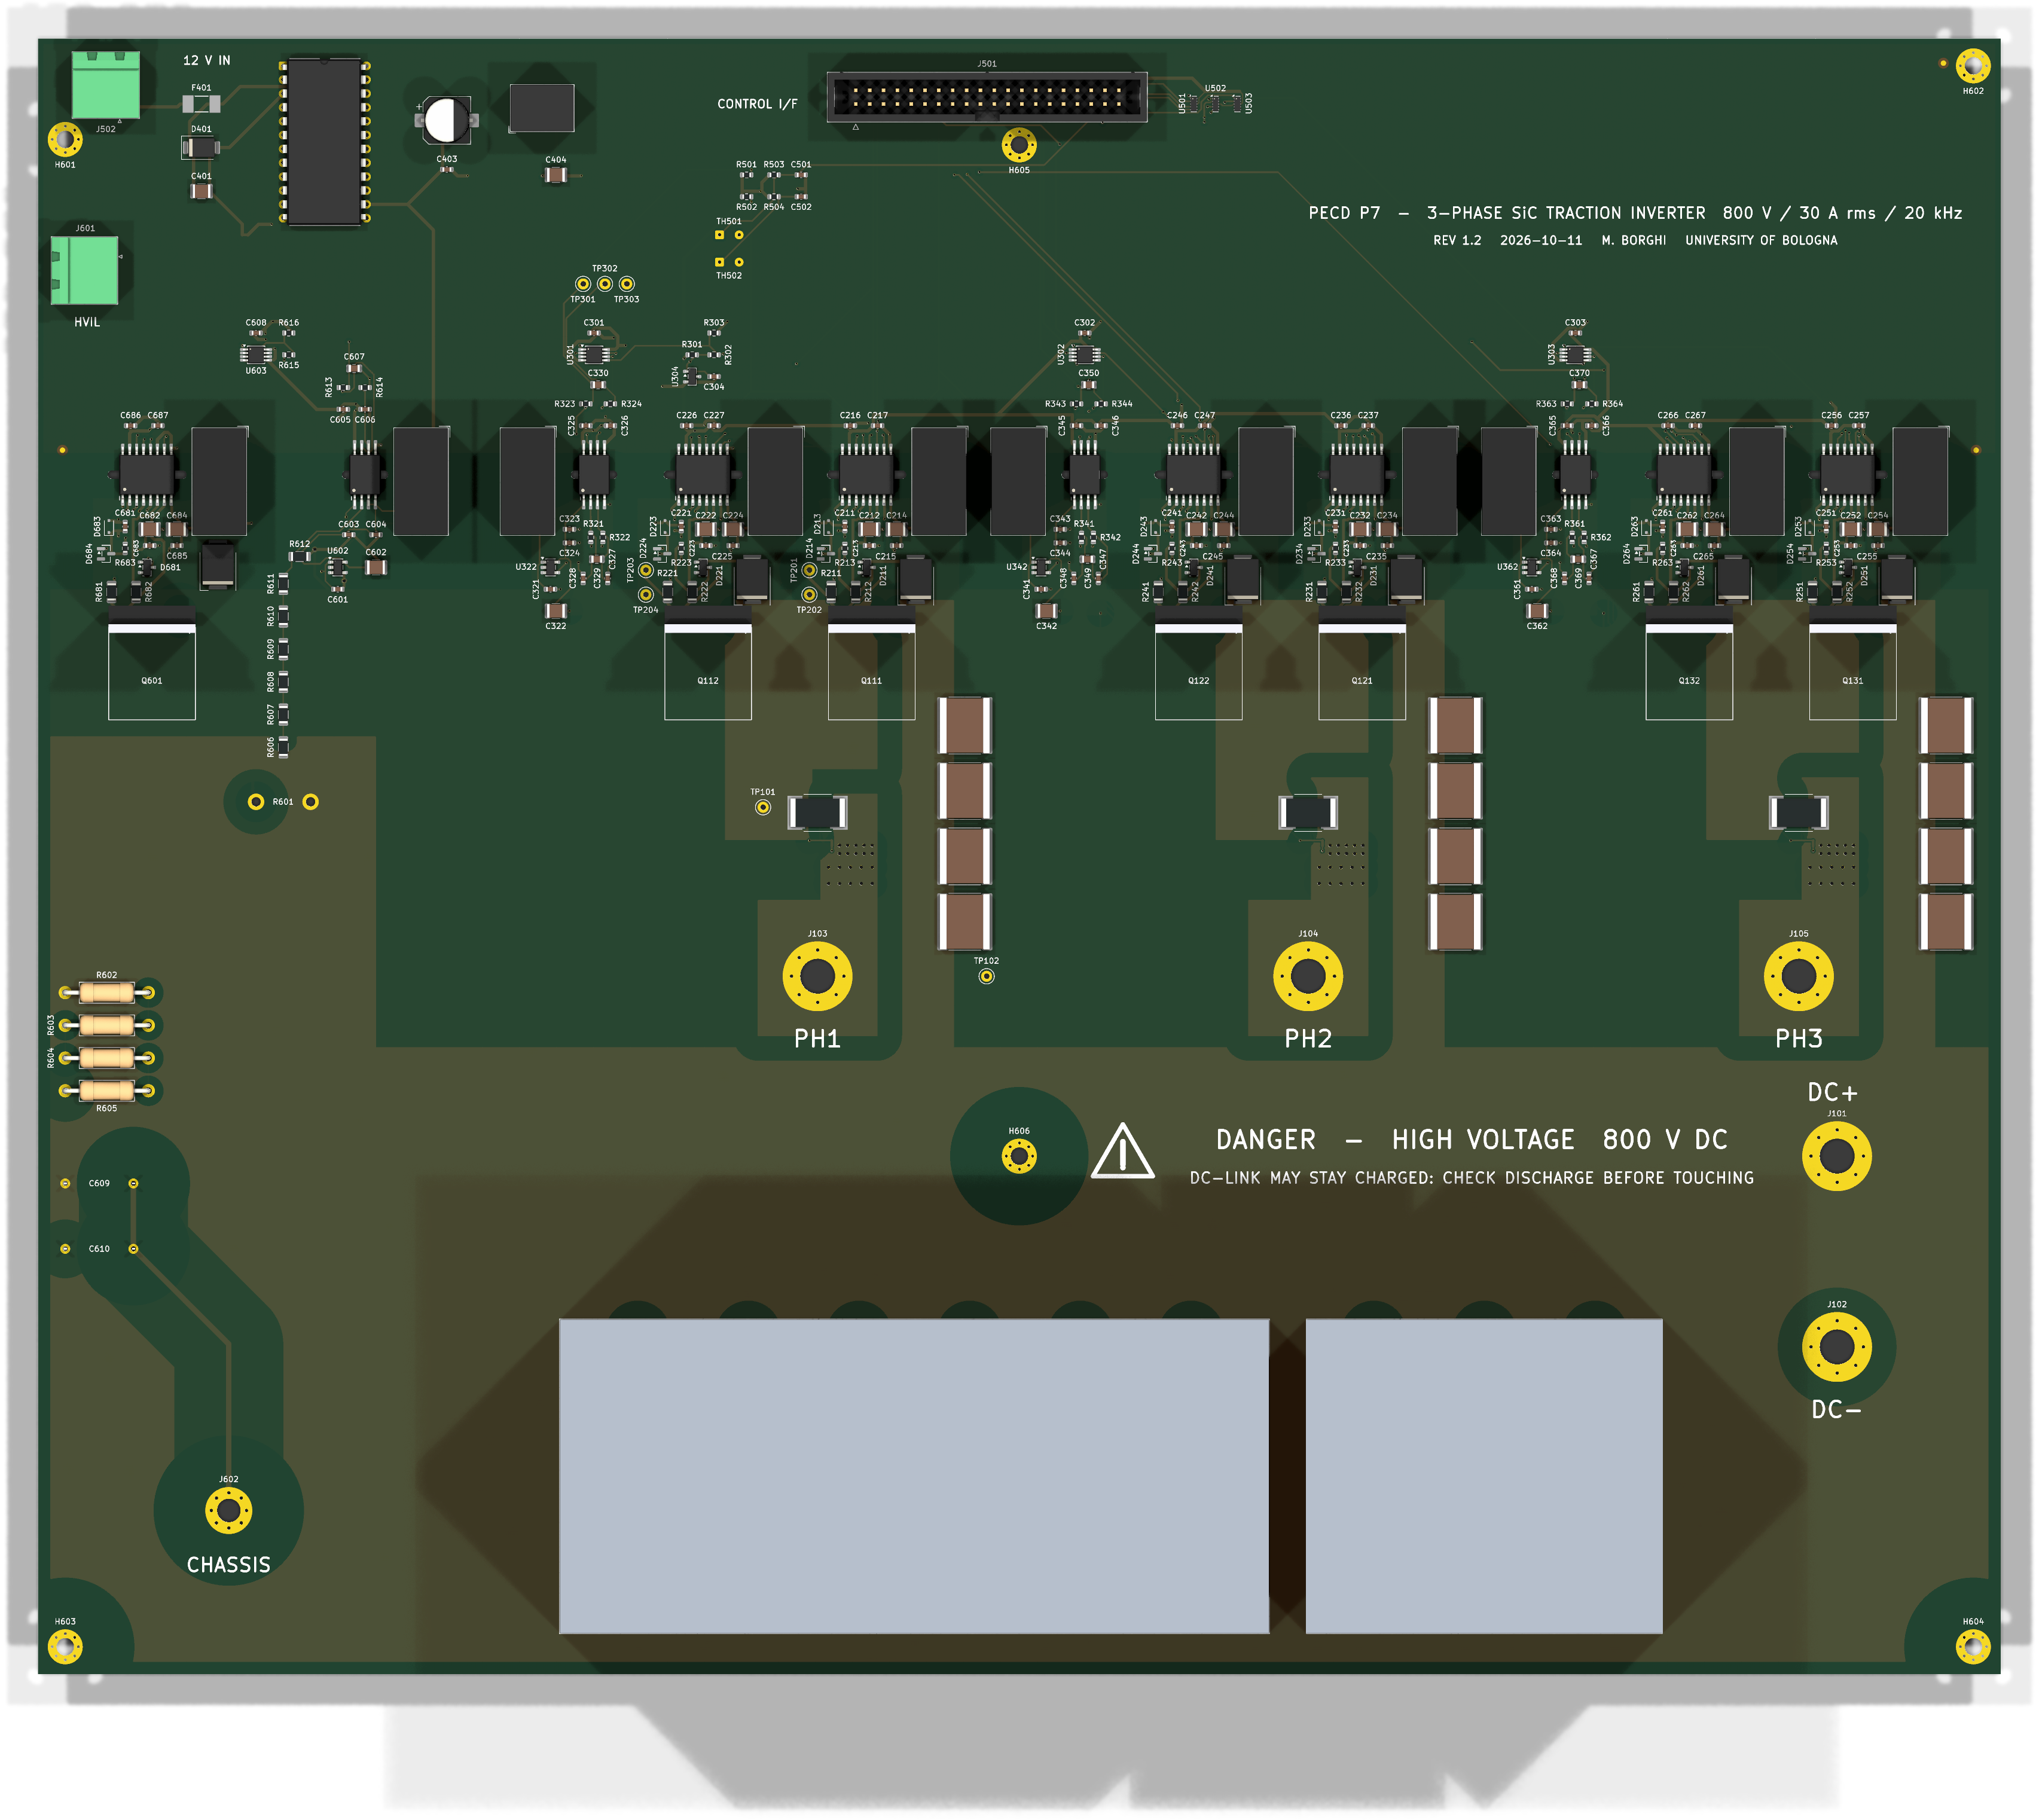
\includegraphics[width=\textwidth]{figures/kicad_3d_alto.png}
  \caption{The board seen from above, \SI{360}{}$\times$\SI{300}{\milli\metre}
  (3D render of the frozen design; bodies of the custom parts are blocks with
  datasheet dimensions). Top to bottom: control connector, auxiliary supply and
  comparators; the row of isolators and isolated supplies astride the barrier;
  the seven TO-247-4L devices and their drivers; phase terminals and
  commutation ceramics; the film DC-link capacitors.}
  \label{fig:pcb-top}
\end{figure}

\begin{figure}[htbp]
  \centering
  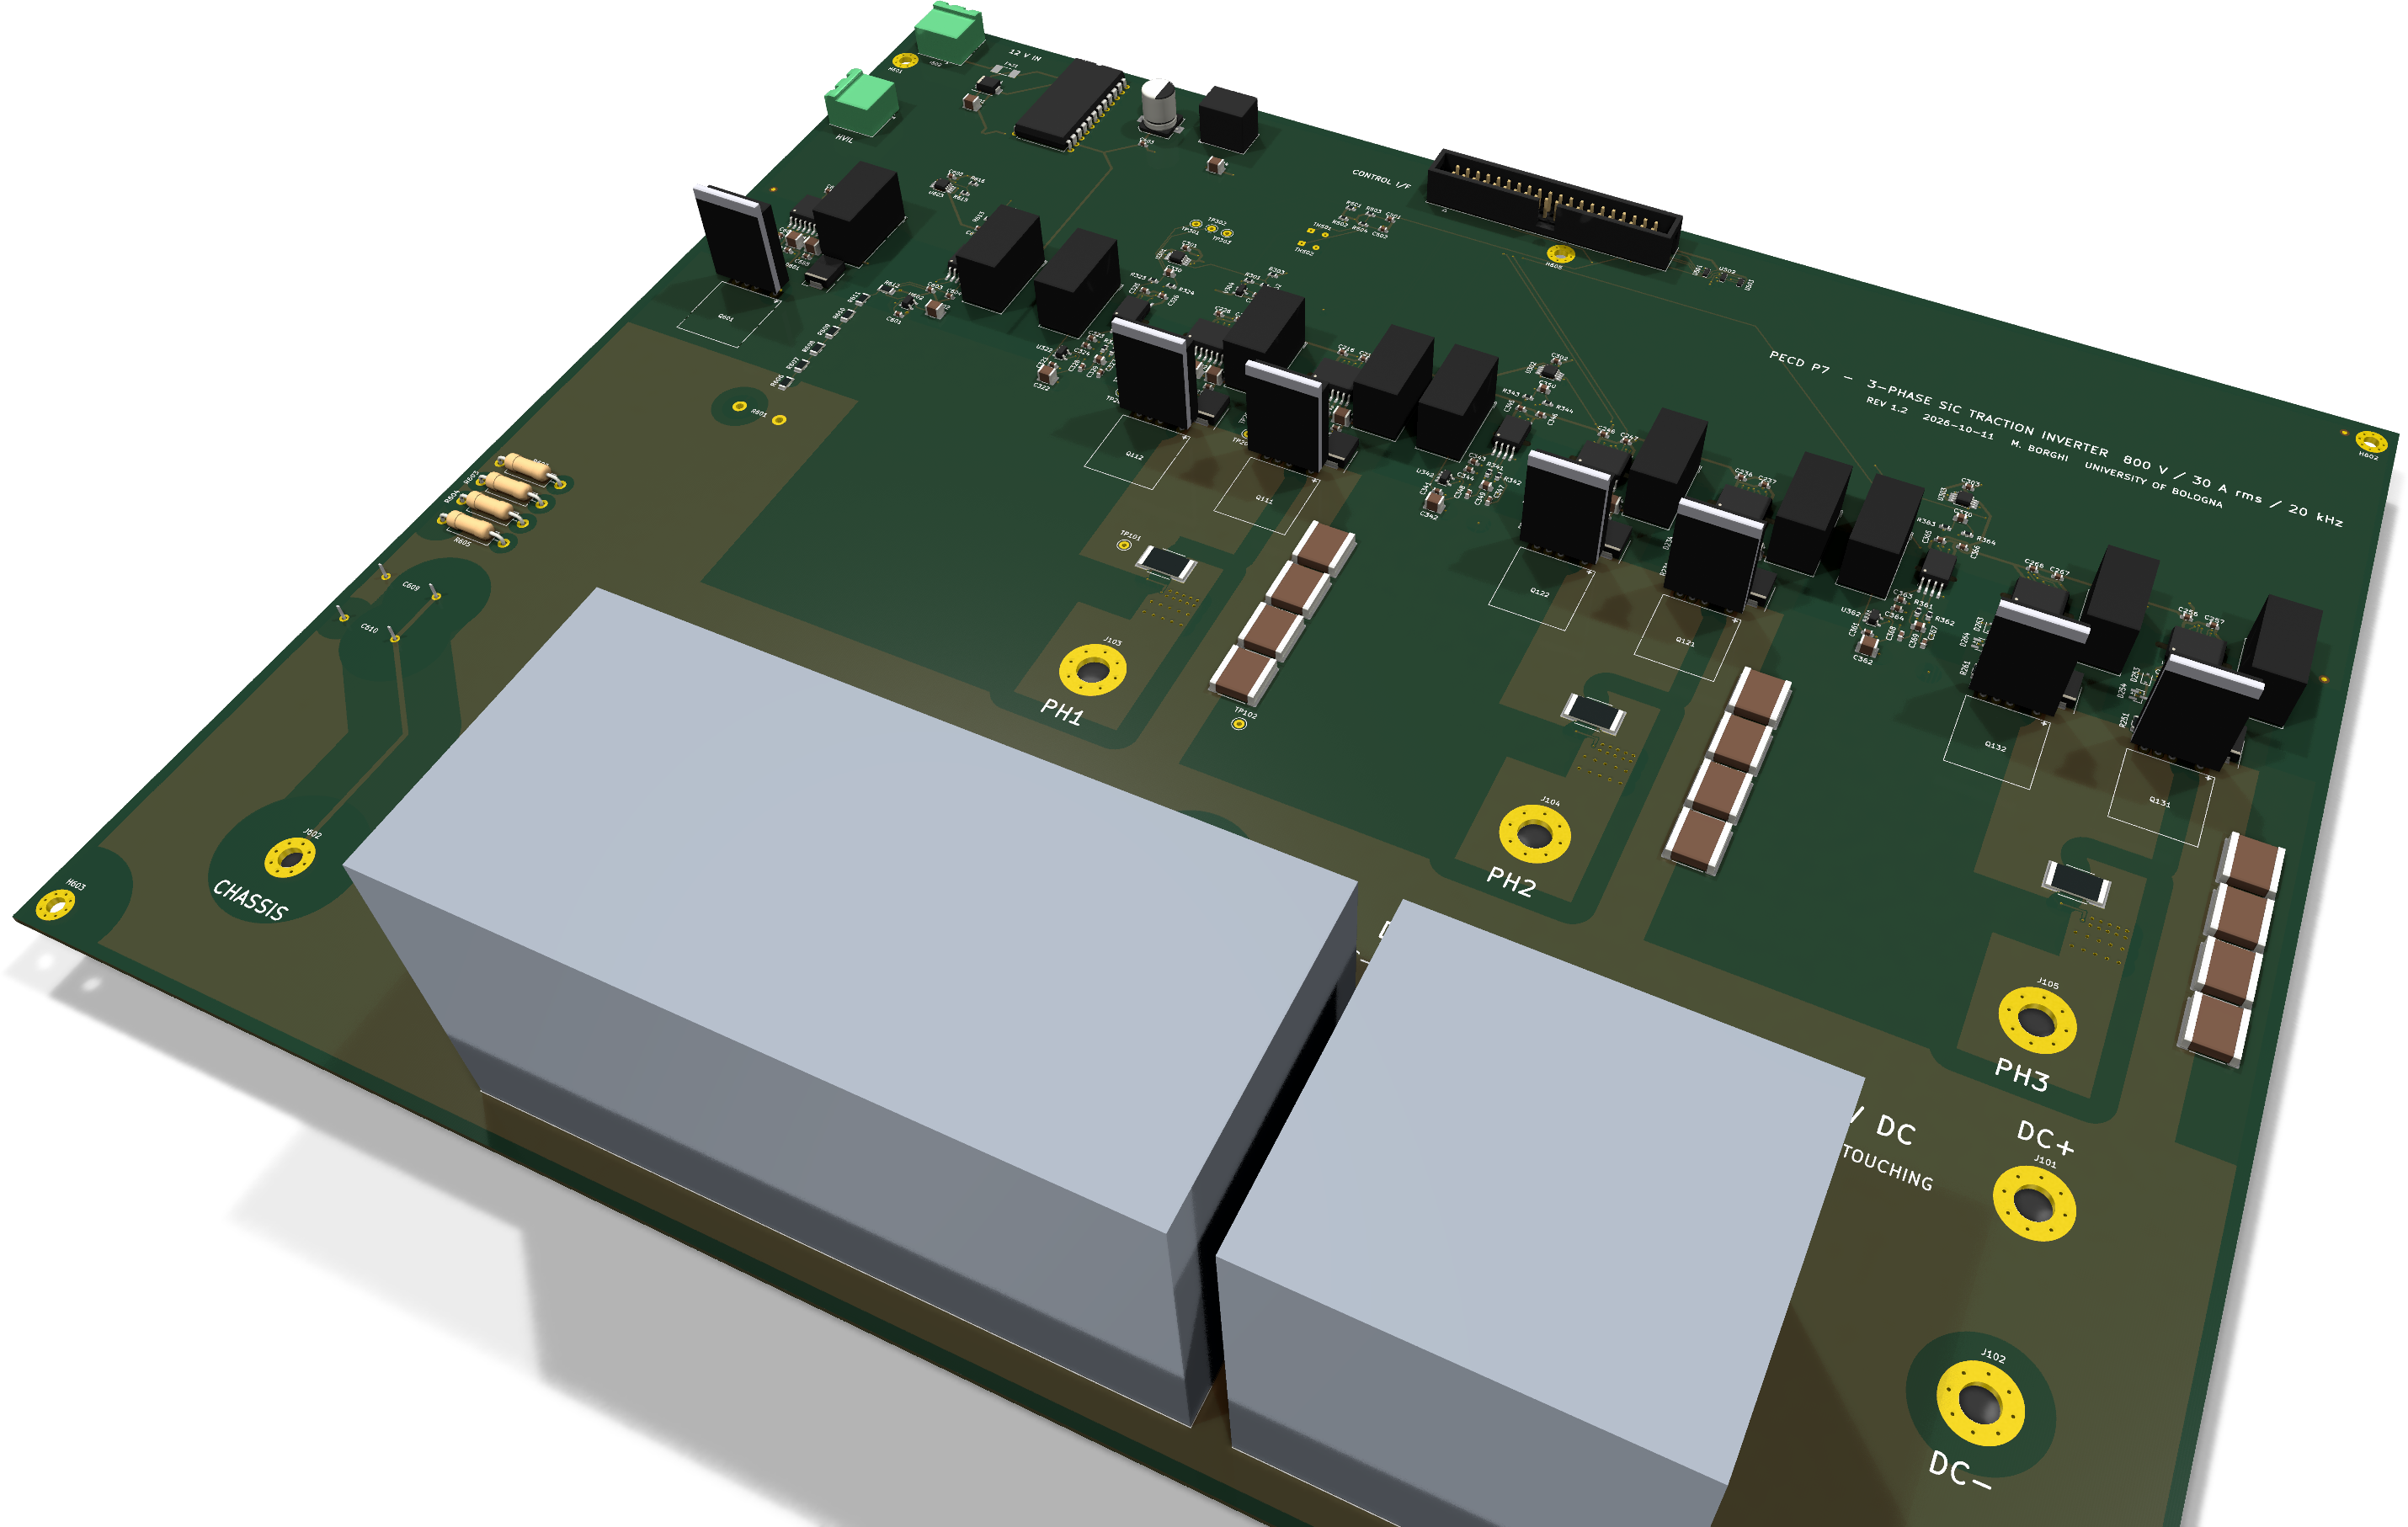
\includegraphics[width=\textwidth]{figures/kicad_3d_iso.png}
  \caption{3D view of the frozen board. The two film capacitors, \SI{65}{\milli\metre}
  tall, occupy the bottom fifth; the TO-247-4L stand vertically, tab towards
  the cold plate.}
  \label{fig:pcb-3d}
\end{figure}

\paragraph{Floorplan.} Everything is on one board
(\cref{fig:pcb-top,fig:pcb-3d}), for three reasons that have numbers behind
them. A connector between a driver board and a power board would add a
pair of parallel pins to every gate loop, about \SI{8}{\nano\henry} for
\SI{10}{\milli\metre} of stacking height; the common-mode current that the
barriers carry, \SI{0.80}{\ampere} peak (\cref{tab:cmcap}), returns on the
board's own ground plane instead of through a cable; and the reinforced
barrier is a single straight line, \SI{80}{\milli\metre} from the top edge,
that every isolator straddles and the design rules check in one piece.
The cost of one board (area that is six-layer even where two layers would
do, and a board lost to any power fault) is accepted for a prototype.

The floorplan follows the domains from top to bottom. The low-voltage side,
above the barrier, carries the control connector, the auxiliary supply, the
overload comparators and the thermistor inputs. On the barrier sit the eleven
isolators (seven \driver{}, three \isoamp{}, one \isoampv{}), each beside its
isolated supply. Below it, each driver faces its own device across a few
millimetres, so the gate loop never leaves its channel. The phase terminals
and the commutation ceramics follow, and the film capacitors fill the bottom
of the board. Six M3 fixing holes, without a net and \SI{9.5}{\milli\metre}
from all high-voltage copper, hold a board of this size against flexing,
which would otherwise fatigue the joints of the film capacitors.

\begin{table}[htbp]
\centering
\caption{The frozen board in numbers.}
\label{tab:boardnumbers}
\small
\begin{tabularx}{\textwidth}{lY}
\toprule
Outline & \SI{360}{}$\times$\SI{300}{\milli\metre}, six layers, \SI{1.6}{\milli\metre} \\
Parts & 275, all on the top side; 271 visible references (the four net ties carry none) \\
Nets & 143, plus 52 single-pin nets of unused pins \\
Tracks & 2168 segments, \SI{8.5}{\metre} in all, every one at \SI{0}{}, \SI{45}{} or \SI{90}{\degree} \\
Vias & 467: 50 on the negative DC rail, 60 stitching the phase pours to L6 \\
Copper pours & positive DC rail on L1 (\SI{411}{\centi\metre\squared}); negative DC plane on L2
  (\SI{627}{\centi\metre\squared}); ground on L3 and L5 (\SI{259}{\centi\metre\squared} each);
  switching nodes and phases on L1; ten floating-reference islands and the three
  phase pours of revision 1.1 on L6 \\
\bottomrule
\end{tabularx}
\end{table}

\paragraph{How the layers are used.} \Cref{fig:layers} shows the six copper
layers. The negative DC plane on L2 lies under the power stage only, and the
two ground planes on L3 and L5 under the low-voltage area only: the two never
overlap in plan, so no high-voltage plane faces a ground plane across a thin
dielectric. L4 carries the signals that cannot stay on the surface, the
sensing pairs among them. L6 carries one copper island per floating domain,
the seven gate references and the four sensing references, each under its
own driver or amplifier; an island is the return path of the gate loop above
it. Since revision 1.1 it also carries a second phase pour under each shunt
(\cref{sec:conductors}).

\begin{figure}[htbp]
  \centering
  \begin{subfigure}{0.49\textwidth}\centering
    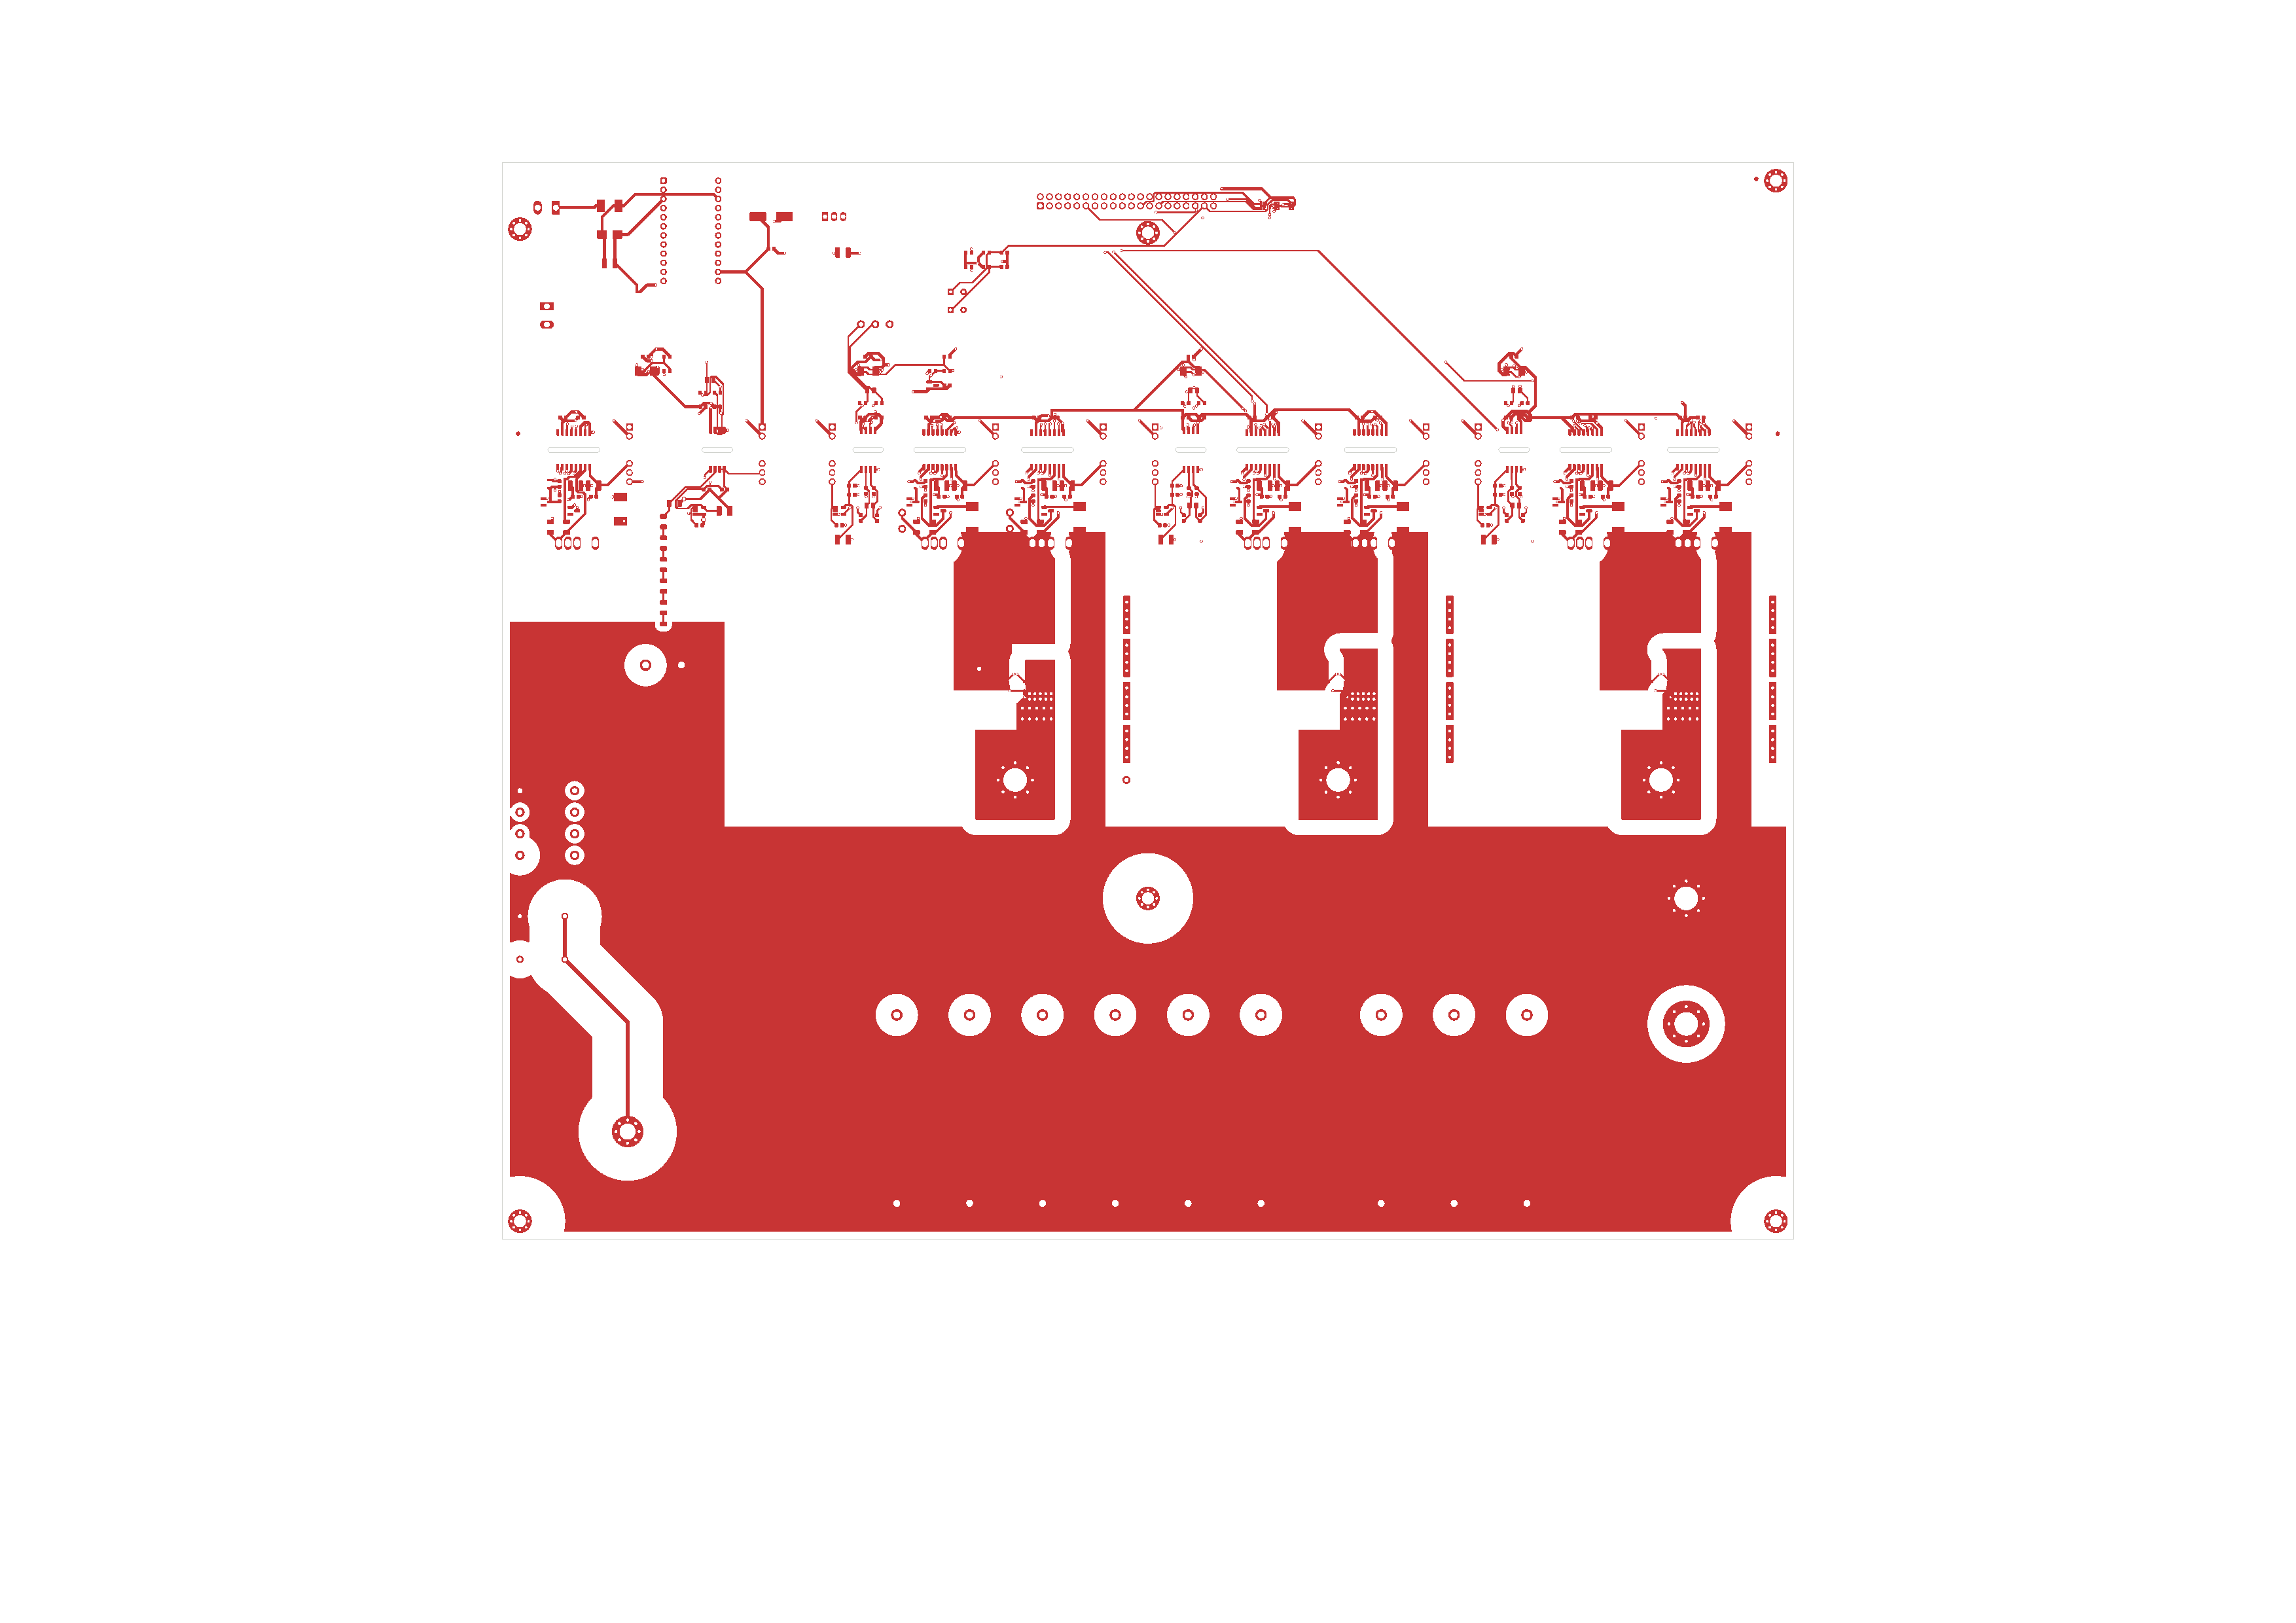
\includegraphics[page=1,width=\textwidth,trim=60mm 40mm 60mm 40mm,clip]{figures/kicad_strati.pdf}
    \caption{L1, top: power pours, components}\end{subfigure}\hfill
  \begin{subfigure}{0.49\textwidth}\centering
    \includegraphics[page=2,width=\textwidth,trim=60mm 40mm 60mm 40mm,clip]{figures/kicad_strati.pdf}
    \caption{L2: negative DC plane, control signals}\end{subfigure}\\[2mm]
  \begin{subfigure}{0.49\textwidth}\centering
    \includegraphics[page=3,width=\textwidth,trim=60mm 40mm 60mm 40mm,clip]{figures/kicad_strati.pdf}
    \caption{L3: ground plane}\end{subfigure}\hfill
  \begin{subfigure}{0.49\textwidth}\centering
    \includegraphics[page=4,width=\textwidth,trim=60mm 40mm 60mm 40mm,clip]{figures/kicad_strati.pdf}
    \caption{L4: signals, sensing pairs}\end{subfigure}\\[2mm]
  \begin{subfigure}{0.49\textwidth}\centering
    \includegraphics[page=5,width=\textwidth,trim=60mm 40mm 60mm 40mm,clip]{figures/kicad_strati.pdf}
    \caption{L5: ground plane}\end{subfigure}\hfill
  \begin{subfigure}{0.49\textwidth}\centering
    \includegraphics[page=6,width=\textwidth,trim=60mm 40mm 60mm 40mm,clip]{figures/kicad_strati.pdf}
    \caption{L6, bottom: floating-reference islands, phase pours}\end{subfigure}
  \caption{The six copper layers of the frozen board.}
  \label{fig:layers}
\end{figure}

\paragraph{Routing.} Every channel was routed once and copied to its twins by
translation, so the seven gate loops are the same copper and the three
sensing channels the same pairs; the local low-voltage nets were routed
partly by an autorouter fed with the class clearances and partly by hand.
Tracks run only at \SI{0}{}, \SI{45}{} and \SI{90}{\degree}.

\begin{figure}[htbp]
  \centering
  \begin{subfigure}{0.48\textwidth}\centering
    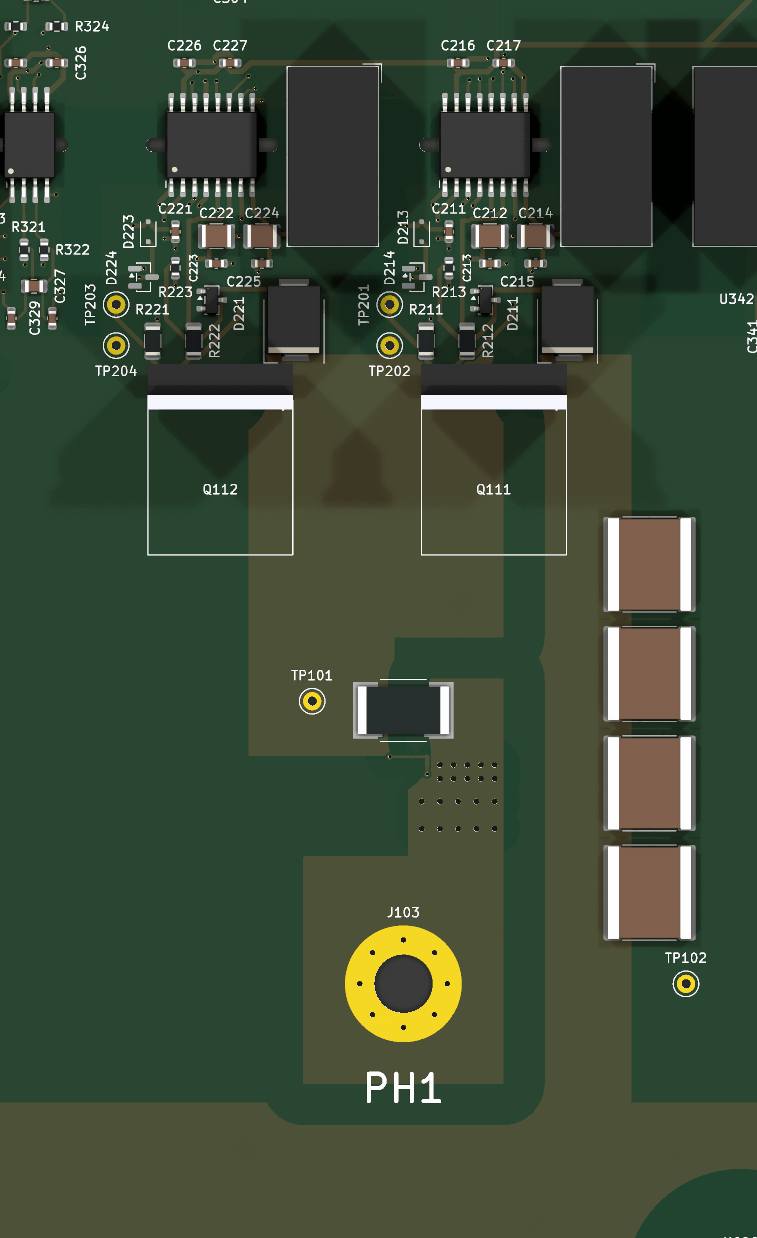
\includegraphics[height=10.5cm,keepaspectratio]{figures/kicad_3d_ramo.png}
    \caption{3D, top}\end{subfigure}\hfill
  \begin{subfigure}{0.48\textwidth}\centering
    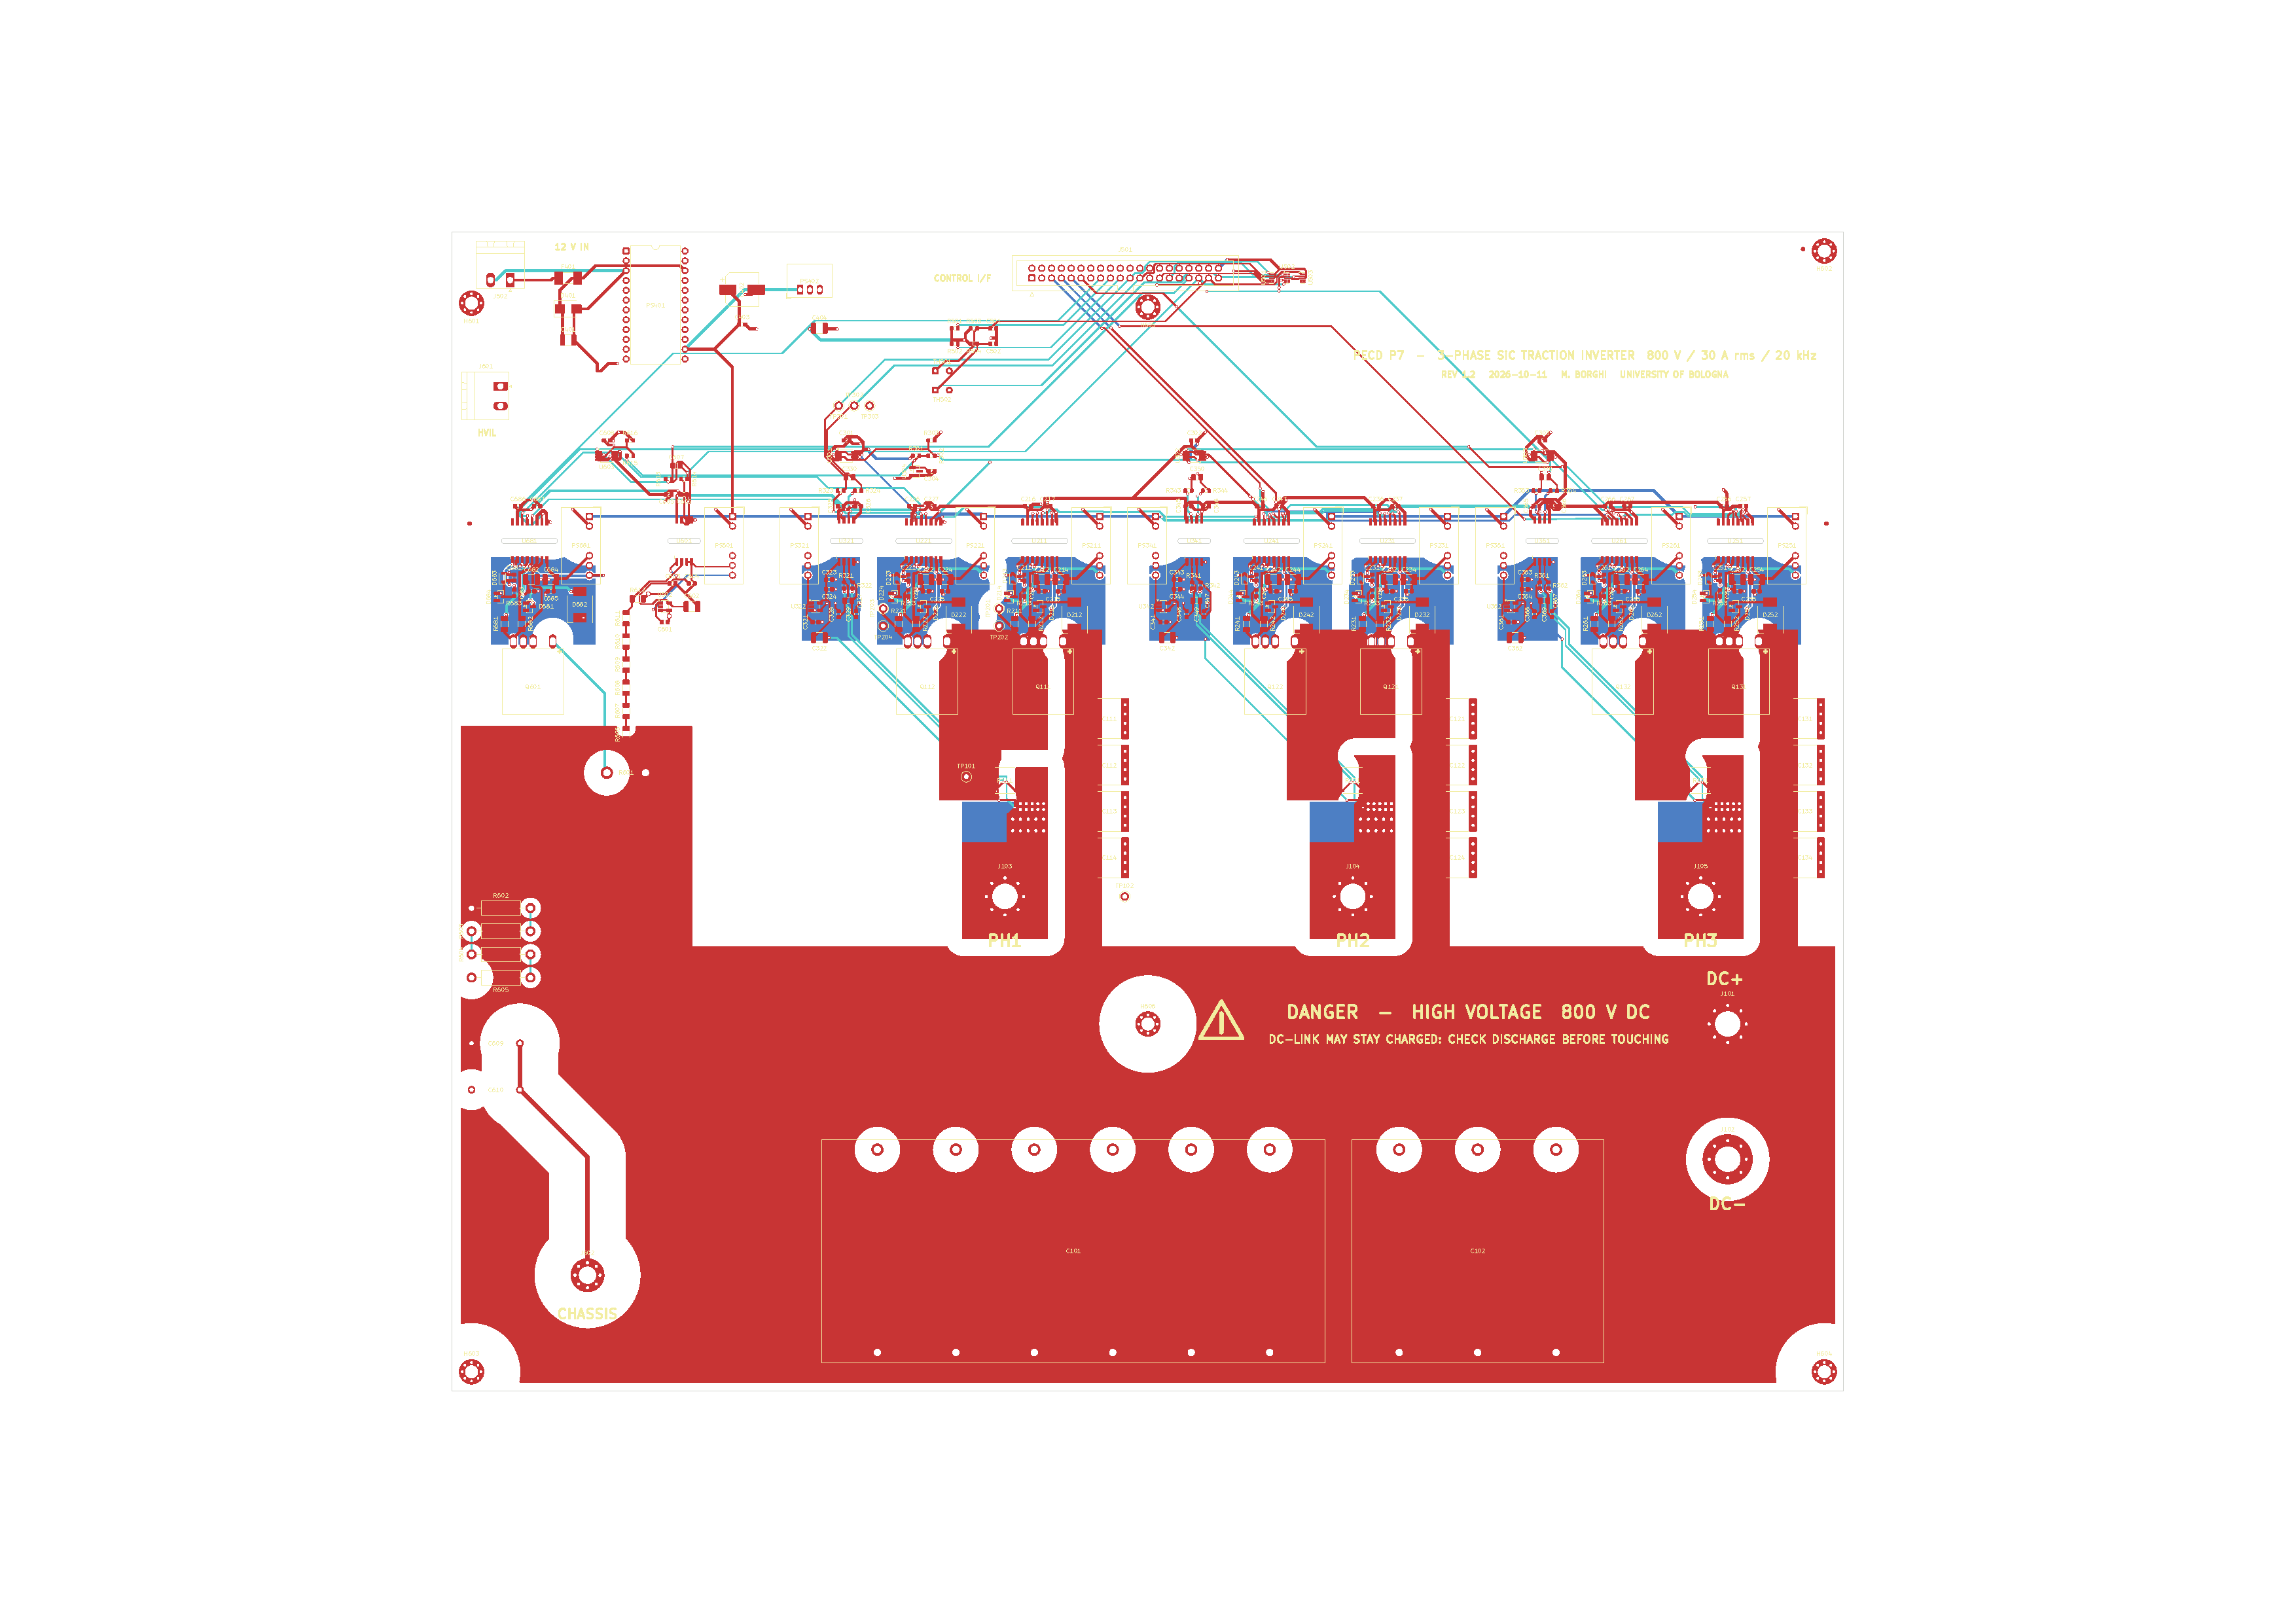
\includegraphics[height=10.5cm,trim=219mm 174mm 295mm 124mm,clip]{figures/kicad_rame_canale.pdf}
    \caption{copper: L1 (red), L4 (cyan), L6 (blue)}\end{subfigure}
  \caption{Leg 1 with its two driver channels: drivers on the barrier, gate
  resistors and desaturation diode between driver and device, the shunt in
  the source path, the four commutation ceramics on the right, the phase
  terminal at the bottom.}
  \label{fig:pcb-leg}
\end{figure}

\paragraph{The gate loop, measured on the copper.} The target of
\SI{25}{\milli\metre} from driver output to gate was set before routing.
Along the tracks of the frozen board it is \SI{23.7}{\milli\metre}
at turn-on and \SI{24.3}{\milli\metre} at turn-off, the same in all seven
channels (\cref{fig:pcb-leg}). The turn-on path dips to L4 through two vias
to clear the parts around the driver; there it runs \SI{0.6}{\milli\metre}
above the reference island on L6 that carries the return, which is closer
than a surface track could get, so the loop is narrower as well as shorter.
Extracted from the copper with the method of \cref{sec:loopextract}, the
loop from the driver output through the gate resistor to the gate, and back
from the Kelvin pin through the island to the driver reference, is
\SI{13}{\nano\henry} (grids of 0.40, 0.30 and
\SI{0.25}{\milli\metre}: 14.3, 13.4, \SI{13.3}{\nano\henry}). That is
consistent with a \SI{0.5}{\milli\metre} track \SI{0.6}{\milli\metre}
above its return, about \SI{0.5}{\nano\henry\per\milli\metre}, and it is
more than the \SI{5}{\nano\henry} the switching simulation had assumed. Its
effect is small (\cref{tab:dptextract}): the gate resistance is above the
critical value $2\sqrt{L/C_\mathrm{iss}}$, so the loop does not ring, and
the peaks move by a few volts.

\paragraph{The sensing pairs.} The two Kelvin connections from each shunt to
its amplifier run side by side on L4, \SI{0.9}{\milli\metre} apart over
\SI{90}{\percent} of their length, \SI{70}{} to \SI{80}{\milli\metre} long.
The two halves of a pair differ in length by up to \SI{8}{\milli\metre}; at
the bandwidth of the measurement that is irrelevant. What matters is the
area enclosed between the two conductors, which picks up the field of the
phase current, and keeping them together keeps it small.

\section{Stack-up}
\label{sec:stackup}

\begin{table}[htbp]
\centering
\caption{Six-layer stack-up, as in the board file. Finished thickness
\SI{1.6}{\milli\metre}.}
\label{tab:stackup}
\begin{tabular}{llll}
\toprule
Layer & Copper & Function & Dielectric below \\
\midrule
L1 & \SI{2}{oz} & power: DC-positive, switching nodes, terminals & prepreg \SI{0.10}{\milli\metre} \\
L2 & \SI{1}{oz} & \textbf{DC-negative plane} (power area); control signals & core \SI{0.46}{\milli\metre} \\
L3 & \SI{1}{oz} & ground plane (low-voltage area) & prepreg \SI{0.20}{\milli\metre} \\
L4 & \SI{1}{oz} & signals: gate turn-on path, sensing pairs, control & core \SI{0.46}{\milli\metre} \\
L5 & \SI{1}{oz} & ground plane (low-voltage area) & prepreg \SI{0.10}{\milli\metre} \\
L6 & \SI{2}{oz} & floating-reference islands of drivers and amplifiers & --- \\
\bottomrule
\end{tabular}
\end{table}

The cores are \SI{0.46}{\milli\metre} rather than the \SI{0.40}{} first
considered, so that the stack adds up to the standard
\SI{1.6}{\milli\metre}; only the L1--L2 prepreg matters electrically, and it
is unchanged.

\paragraph{Six layers or four.} Before routing, a four-layer board looked
equivalent: the negative DC plane and the ground planes never overlap in
plan, so they could have shared one layer, with one signal layer below it.
The routed board uses both inner signal layers: L4 carries
\SI{3.4}{\metre} of track (the turn-on half of every gate loop and all the
sensing pairs among it), and L2 another \SI{1.2}{\metre} of control signals
above the barrier. A four-layer version would have to fit both into one
layer and keep a single ground plane under the control area. That was not
attempted, so the six layers are justified by the density the routing
reached, not proven necessary; at a production cost review it is the first
thing to try.

The one dimension that the stack-up exists to fix is the L1--L2 prepreg. Two
facing planes carrying a current and its return have
%
\begin{equation}
  L = \frac{\mu_0\,h\,l}{w},
  \label{eq:planepair}
\end{equation}
%
proportional to the separation $h$. For the \SI{30}{\milli\metre} by
\SI{20}{\milli\metre} region that the commutation loop occupies:

\begin{table}[htbp]
\centering
\caption{Plane-pair inductance against prepreg thickness,
$l = \SI{30}{\milli\metre}$, $w = \SI{20}{\milli\metre}$.}
\label{tab:planepair}
\begin{tabular}{lr}
\toprule
L1--L2 separation & Inductance \\
\midrule
\SI{0.075}{\milli\metre} & \SI{0.141}{\nano\henry} \\
\SI{0.10}{\milli\metre} (selected) & \SI{0.188}{\nano\henry} \\
\SI{0.20}{\milli\metre} & \SI{0.377}{\nano\henry} \\
\SI{0.36}{\milli\metre} (standard core) & \SI{0.679}{\nano\henry} \\
\bottomrule
\end{tabular}
\end{table}

\begin{finding}{The plane pair is not where the inductance budget is spent}
Against a target of \SI{20}{\nano\henry} the plane pair contributes under
\SI{0.7}{\nano\henry} even with a standard \SI{0.36}{\milli\metre} core. The
thin prepreg is still specified, because it costs nothing and every tenth of
a nanohenry saved stays available elsewhere, but it is not the decisive
choice. The budget is spent on vertical transitions (vias, pads, the leads
between board and device) and on the path to the ceramic capacitors.

A corollary follows: if \SI{0.10}{\milli\metre} ever
becomes awkward, doubling it costs \SI{0.19}{\nano\henry} and halves the
electric stress in the solid insulation from \SI{9}{} to
\SI{4.5}{\kilo\volt\per\milli\metre} at \SI{900}{\volt}
(\cref{sec:insulation}). That is a good
trade, and it should be reconsidered at the first prototype.
\end{finding}

\begin{table}[htbp]
\centering
\caption{Commutation loop budget, estimated before layout; the last rows
give the extraction from the frozen board (\cref{sec:loopextract}).}
\label{tab:loopbudget}
\small
\begin{tabular}{lrl}
\toprule
Contribution & [\si{\nano\henry}] & Controlled by layout? \\
\midrule
Device packages & 14.6 & no \\
Leads and pads & 3--6 & partly: short leads \\
Vias and vertical transitions & 0.4--2 & yes \\
Plane pair L1--L2 & 0.19 & yes, and already negligible \\
Ceramic capacitor ESL & 1--2 & yes: more parts in parallel \\
\midrule
\textbf{Board-attributable total} & \textbf{5--10} & target \SI{20}{\nano\henry}: reachable \\
\textbf{Physical loop} & \textbf{20--25} & \\
\midrule
Extracted, revision 1.0: board copper & 12$\pm$1 & three legs alike \\
\quad of which at the clearance holes & 7.7 & yes: inner-layer clearance \\
\textbf{Extracted, revision 1.1: board copper} & \textbf{7.8} & inner-layer clearance relaxed \\
\textbf{Revision 1.1, with capacitor ESL} & \textbf{about 8.3} & \SI{14}{\nano\henry} to the C2 threshold \\
\bottomrule
\end{tabular}
\end{table}

\section{Commutation loop}

The limit is \SI{20}{\nano\henry} of PCB-attributable inductance and the
failure threshold \SI{22.6}{\nano\henry}. The limit is a design input: the gate resistances of \SI{5}{}/\SI{12.5}{\ohm} were
chosen so that the die stays below \SI{1080}{\volt} at \SI{950}{\volt} and
\SI{60}{\ampere} \emph{with} \SI{20}{\nano\henry} (\cref{sec:kelvin}). The
frozen board's loop is extracted below (\cref{sec:loopextract}) and still
to be measured (test B2 of \cref{tab:benchplan}); both are to be checked
against the threshold at which C2 is
lost, \SI{22.6}{\nano\henry} at turn-off and
\SI{23.6}{\nano\henry} on recovery (\cref{tab:lthreshold}), not only
against the limit: the \SI{2.6}{\nano\henry} between them is the whole
margin, and above \SI{23}{\nano\henry} the recovery peak rises four times
faster than the turn-off one. As established there, the device packages contribute a
further \SI{14.6}{\nano\henry} that no layout can remove, so the physical
loop will measure around \SI{35}{\nano\henry} at the limit and
\SIrange{20}{25}{\nano\henry} at the estimate of \cref{tab:loopbudget}.

\subsection{Extracted from the copper of the frozen board}
\label{sec:loopextract}

\paragraph{Method.} The loop of this board is made of pours, not tracks: the
positive rail and the switching node on L1, the negative plane on L2,
\SI{0.10}{\milli\metre} below. A track-based extraction does not see it,
so the copper of each leg was extracted with the partial-element method
that FastHenry uses. The filled copper of L1 and L2 is read from the board
file on a square grid; every pair of parallel cells has a mutual partial
inductance, computed in closed form along the cell and by integration
across it; the high-side device and each ceramic are ideal shorts between
their pads, and the loop is seen from the drain--source terminals of the
low-side device. Resistance is neglected, which is the high-frequency limit
that matters for the switching edge. The result is the \emph{board}
contribution, to which the packages (\SI{14.6}{\nano\henry}, in the
vendor's model) and the capacitor ESL are added.

The solver was checked before it was trusted: two parallel plates
\SI{10}{}$\times$\SI{30}{\milli\metre} at \SI{0.10}{\milli\metre} give
\SI{0.355}{\nano\henry} against \SI{0.364}{\nano\henry} from
\cref{eq:planepair}, the small deficit being the fringing the formula
ignores; a square loop of strip, a case with no plane at all, matches its
closed form within \SI{1}{\percent}. On the board, grids from
\SI{1.25}{} to \SI{0.8}{\milli\metre} give 11.7 to \SI{12.7}{\nano\henry}
without a trend, the scatter coming from how the pins fall on the grid.

\paragraph{Result.} Revision 1.0 gave \SI{12}{}$\pm$\SI{1}{\nano\henry} of
board copper, the same in the three legs, which are copies; the finding
below explains where it was spent and why revision 1.1 brings it to
\SI{7.8}{\nano\henry} (\SI{8.2}{\nano\henry} on the finer grid). The
ceramic datasheet gives no ESL; from the geometry of the body over the
plane, four in parallel add about \SI{0.5}{\nano\henry}. The
board-attributable loop of the frozen board is therefore about
\SI{8.3}{\nano\henry}: well below the \SI{20}{\nano\henry} on which the gate
resistances were chosen and \SI{14}{\nano\henry} from the
\SI{22.6}{\nano\henry} at which C2 is lost. The physical loop, packages
included, is about \SI{23}{\nano\henry}.

\paragraph{The switching simulation with the extracted values.} The
double-pulse bench of \cref{sec:kelvin} was run again with the extracted
loop and gate-loop inductances in place of the budget, and nothing else
changed; it reproduces the report's case exactly when given the budget.

\begin{table}[htbp]
\centering
\caption{Double pulse at \SI{950}{\volt}, \SI{60}{\ampere}, \SI{175}{\celsius},
$R_g$ \SI{5}{}/\SI{12.5}{\ohm}: the budget against the extracted board.
Peak at the die; limit \SI{1080}{\volt}.}
\label{tab:dptextract}
\small
\begin{tabular}{lrrrr}
\toprule
Case & Loop & Gate loop & Turn-off peak & Recovery peak \\
\midrule
Budget (\cref{sec:kelvin}) & \SI{20}{\nano\henry} & \SI{5}{\nano\henry} & \SI{1073.5}{\volt} & \SI{1050.0}{\volt} \\
Revision 1.0, extracted & \SI{12.5}{\nano\henry} & \SI{13}{\nano\henry} & \SI{1052.5}{\volt} & \SI{1046.6}{\volt} \\
\textbf{Revision 1.1, extracted} & \SI{8.3}{\nano\henry} & \SI{13}{\nano\henry} & \textbf{\SI{1040.1}{\volt}} & \SI{1027.2}{\volt} \\
\bottomrule
\end{tabular}
\end{table}

The margin at the die goes from \SI{6.5}{} to \SI{40}{\volt}. It could be
spent: with the extracted loop, $R_{g,\mathrm{off}}$ could come down to
\SI{7.5}{\ohm} with the die at \SI{1064}{\volt}, and the model's turn-off
energy would fall by \SI{38}{\percent}; at \SI{5}{\ohm} the die reaches
\SI{1087}{\volt} and C2 is lost. The resistor is not changed. The
margin comes from a model of the copper, not from a measurement, and
spending it before test B2 has confirmed it would stake the most expensive
part on the board on an unverified number. It is the first change to make
once the loop has been measured.

\begin{figure}[htbp]
  \centering
  \begin{subfigure}{\textwidth}\centering
    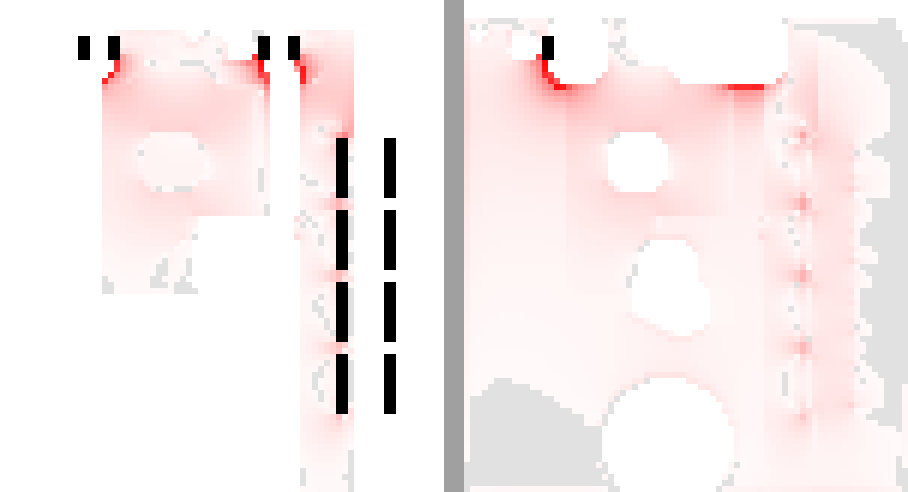
\includegraphics[width=0.92\textwidth]{figures/kicad_maglia_energia_v10.png}
    \caption{revision 1.0: \SI{11.7}{\nano\henry}}\end{subfigure}\\[2mm]
  \begin{subfigure}{\textwidth}\centering
    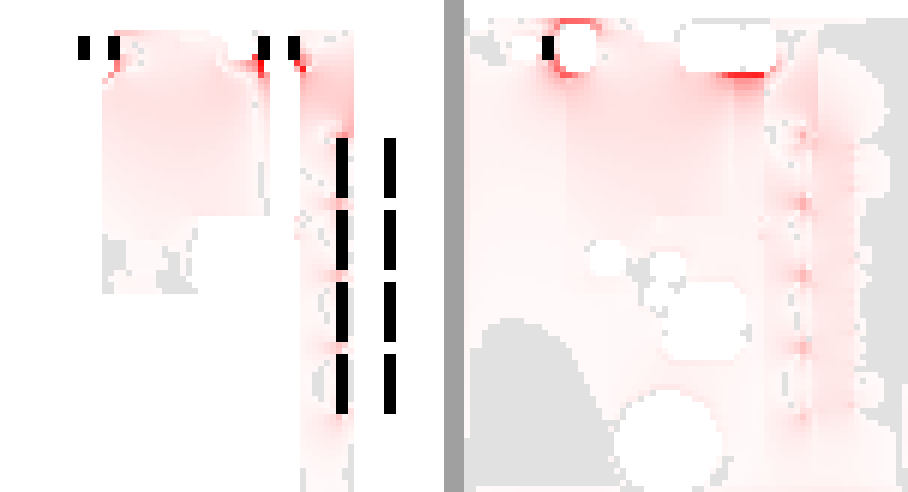
\includegraphics[width=0.92\textwidth]{figures/kicad_maglia_energia_v11.png}
    \caption{revision 1.1, inner-layer clearance \SI{2.25}{\milli\metre}: \SI{7.8}{\nano\henry}}\end{subfigure}
  \caption{Magnetic energy density of the commutation loop of leg~1 at
  \SI{1}{\milli\metre} resolution, L1 on the left, L2 on the right of each
  pair (black: device and capacitor pads; grey: copper carrying little
  energy; same colour scale within each pair). The energy sits at the device
  pins and along the edges of the clearance holes that the negative plane
  leaves around the other pins; smaller holes, less energy.}
  \label{fig:loopenergy}
\end{figure}

\begin{finding}{The inductance is in the clearance holes, not in the plane pair}
The estimate of \cref{tab:loopbudget} was 5 to \SI{10}{\nano\henry}; the
extraction of revision 1.0 gave more, and \cref{fig:loopenergy} shows where. Of the
\SI{12}{\nano\henry}, \SI{8.6}{} are spent in the strip of board under the
device row, and almost all of it along the edges of the holes in the
negative plane. The plane must keep \SI{4.5}{\milli\metre} from the
switching-node and positive-rail pins and from the high-side gate pins,
which on a \SI{5.08}{\milli\metre} pitch opens a hole about
\SI{10}{\milli\metre} wide under each device: the return current has to
drop some \SI{6}{\milli\metre} below the row before it can run under the
outgoing current. With a plane free of holes (not buildable, but a useful
bound) the same copper gives \SI{4.0}{\nano\henry}; the holes cost
\SI{7.7}{\nano\henry}.

The \SI{4.5}{\milli\metre} is a creepage figure for a surface in
pollution degree 2, and it is applied to every layer. Inside the laminate
there is no surface and no pollution: IPC-2221B asks
\SI{0.0025}{\milli\metre\per\volt} above \SI{500}{\volt} for internal
conductors, \SI{2.25}{\milli\metre} at \SI{900}{\volt}~\cite{ipc2221}. Applied
to the inner layers only, it takes the loop from 12 to
\SI{7.8}{\nano\henry}, a third less, with no other change to the copper.
Revision 1.1 adopts it: one rule, for the negative plane against
the other high-voltage nets and the high-side domains on inner layers; the
outer layers keep \SI{4.5}{\milli\metre} and the reinforced barrier is
untouched. Four new cases on the rules test board check exactly that (2 and
\SI{3}{\milli\metre} on L2, \SI{3}{\milli\metre} on L1,
\SI{6}{\milli\metre} to ground on L2).
\end{finding}

\section{Conductor sizing}
\label{sec:conductors}

Two currents have to be carried. The phase conductors carry
\SI{30}{\Arms}; the DC bus carries the input current
%
\begin{equation}
  I_\mathrm{bus} = \frac{P_\mathrm{out} + P_\mathrm{tot}}{\Vdc}
  = \frac{\SI{25.605}{\kilo\watt}}{\SI{800}{\volt}}
  = \SI{32.0}{\ampere},
  \label{eq:ibus}
\end{equation}
%
rounded up to \SI{35}{\ampere} for the ripple superimposed on it.

\begin{table}[htbp]
\centering
\caption{Minimum conductor width, IPC-2221B closed form~\cite{ipc2221},
external layer, \SI{2}{oz} copper.}
\label{tab:widths}
\begin{tabular}{llrr}
\toprule
Conductor & Current & $\Delta T = \SI{20}{\kelvin}$ & $\Delta T = \SI{30}{\kelvin}$ \\
\midrule
Phase  & \SI{30}{\Arms}   & \SI{10.7}{\milli\metre} & \SI{8.4}{\milli\metre} \\
DC bus & \SI{35}{\ampere} & \SI{13.3}{\milli\metre} & \SI{10.4}{\milli\metre} \\
\bottomrule
\end{tabular}
\end{table}

At these currents the conductors are copper pours, not tracks, and the
computed widths serve as a minimum check. Two warning rules flag any
\emph{track} on a bus or phase net narrower than \SI{10.4}{} or
\SI{8.4}{\milli\metre}. Two kinds of connection are exempted by name,
because they carry milliamperes and not the load current: the desaturation
diode's lead to the drain, and the bus-voltage divider around the bus
amplifier, marked by a rule area. Every other narrow track on those nets
still raises the warning, and the frozen board raises none.

\begin{finding}{The width rule checks tracks, and the narrowest conductor is a pour}
The positive DC rail is a single pour of \SI{411}{\centi\metre\squared} on
L1 over the \SI{627}{\centi\metre\squared} negative plane on L2, and the
switching-node pours are never narrower than \SI{13}{\milli\metre}. The
phase pours were measured afterwards, section by section on the filled
copper, because no rule looks at them: they are at least
\SI{10.5}{\milli\metre} wide from the shunt to the terminal, but
about \SI{8}{\milli\metre} for some \SI{4}{\milli\metre} just below
the shunt pad, where the pour of the switching node takes the rest of the row.

That is below the \SI{8.4}{\milli\metre} of the \SI{30}{\kelvin} column; by
the same closed form a long conductor that narrow would rise by about
\SI{33}{\kelvin} instead of \SI{30}{}. Revision 1.1 removes the
neck without moving a part: a second phase pour on L6, the full
\SI{22}{\milli\metre} of the phase area wide because the switching node has
no copper on that layer, stitched to L1 by twenty vias in four rows and
collected at the phase terminal, which is through-hole. The narrowest
section becomes 8 plus \SI{22}{\milli\metre} of \SI{2}{oz} copper. The pour
starts \SI{5.5}{\milli\metre} below the shunt centre, so the phase current
on L6 does not run under the Kelvin loop of the measurement. Widening the
L1 pour instead would have meant relaxing the \SI{4.5}{\milli\metre}
between switching node and phase, two nets a few millivolts apart in
operation but not if the shunt fails open. The lesson is about the check
rather than the copper: a width rule on tracks says nothing about pours,
and a board whose power path is all pours needs its sections measured.
\end{finding}

The IPC-2152 charts~\cite{ipc2152} supersede the closed form and were not
available (\cref{app:assumptions}, A.15).

\section{Common-mode and EMC}
\label{sec:emc}

Emissions can only be measured against CISPR 25~\cite{cispr25} on a built
board; what the layout can do is keep the common-mode currents short and
known. The switching node moves the full bus at \SI{31}{\volt\per\nano\second}
between \SI{10}{} and \SI{90}{\percent} of the steeper edge, in the
double-pulse simulation at \SI{950}{\volt} and \SI{60}{\ampere}
(\cref{sec:kelvin}), and every capacitance to chassis carries a current
proportional to that slope.

\begin{table}[htbp]
\centering
\caption{Capacitance from the switching nodes to chassis.}
\label{tab:cmcap}
\begin{tabular}{lrr}
\toprule
Source & Capacitance & Peak current \\
\midrule
Isolation barriers of the auxiliary circuits & \SI{25.5}{\pico\farad} & \SI{0.80}{\ampere} \\
\textbf{Insulating pads, three low-side devices} & \SI{131}{\pico\farad} & \SI{4.11}{\ampere} \\
Motor and cable, assumed & \SI{1}{\nano\farad} & \SI{31}{\ampere} \\
\bottomrule
\end{tabular}
\end{table}

The middle row was missing from the earlier analysis. The pad is an
insulator and a capacitor at once: alumina of relative permittivity
\num{9.8}, \SI{0.63}{\milli\metre} thick, under a
\SI{15.9}{}$\times$\SI{20}{\milli\metre} tab gives \SI{43.8}{\pico\farad} per
device. Only three of the six count, because the tab is the \emph{drain}: on
the high side that is the DC-positive rail, which does not move, and on the
low side it is the switching node, which does. The aluminium nitride
adopted in \cref{sec:coolalt} has a permittivity of about 
\num{8.8}, ten
percent less: the alumina figures are kept here as the upper bound.

The conclusion survives, since the motor cable still dominates and effort
belongs in the screen termination and the Y-capacitors, but by a factor of
\num{7.6} rather than \num{40}, and second place belongs to the pads rather
than to the driver barriers. If on-board common-mode current had to be
reduced, the lever would be a \emph{thicker} pad, not a lower-capacitance
driver: halving the thickness doubles this term to
\SI{263}{\pico\farad} while halving $\Rthcs$. Pad \emph{area} does not enter
it at all, since the electrode is the tab and the fringing field decays over
a distance of order the thickness, and the \SI{8.4}{\milli\metre} overhang
is already thirteen times that.

\subsection{A first estimate against CISPR 25}
\label{sec:emcest}

Emissions are measured, not computed; but the two sources that drive the
conducted part are known well enough to say, before a board exists, how far
from a limit it will start and what filter it will need. The estimate works
on a circuit model of the measurement set-up of CISPR~25~\cite{cispr25}: the
\SI{5}{\micro\henry}/\SI{50}{\ohm} artificial network on each DC line, a
metre of harness, and the impedances this report has already computed.
%
\begin{itemize}
  \item The sources, simulated with the real modulation over one
        fundamental period: the common-mode voltage of the three legs and the
        input current of the bridge, with the edges of the double-pulse
        simulation. Two operating points: rated, and locked rotor, where the
        three duty cycles are almost equal, the legs switch together and the
        common-mode voltage is the worst it can be.
  \item The paths: for the common mode, the capacitances to chassis of
        \cref{tab:cmcap} and the two Y-capacitors that return the current to
        the bus; for the differential mode, the commutation ceramics, the
        films behind the plane inductance, and the harness.
  \item The receiver: a \SI{9}{\kilo\hertz} Gaussian filter and a peak
        detector, compared with the voltage-method peak limits of the
        broadcast bands, class~3 as reference. These are the low-voltage
        limits; the edition and class for the high-voltage lines remain to be
        fixed (A.19), so the comparison says how large the gap is, not whether
        a test passes.
\end{itemize}

\begin{table}[htbp]
\centering
\caption{Estimated conducted emission above the CISPR~25 class~3 peak limit,
worst operating point, by band (dB; negative is below the limit).}
\label{tab:emcest}
\small
\begin{tabular}{lrrrr}
\toprule
 & LW & MW & SW & CB \\
Band [\si{\mega\hertz}] & 0.15--0.3 & 0.53--1.8 & 5.9--6.2 & 26--28 \\
\midrule
Common mode, board as frozen & $+19$ & $+56$ & $+35$ & $+8$ \\
Differential mode, board as frozen & $-3$ & $+33$ & $-1$ & $-13$ \\
Common mode, with the input filter & $-9$ & $-3$ & $-3$ & $-7$ \\
Differential mode, with the input filter & $-34$ & $-33$ & $-69$ & $-80$ \\
\bottomrule
\end{tabular}
\end{table}

\begin{figure}[htbp]
\centering
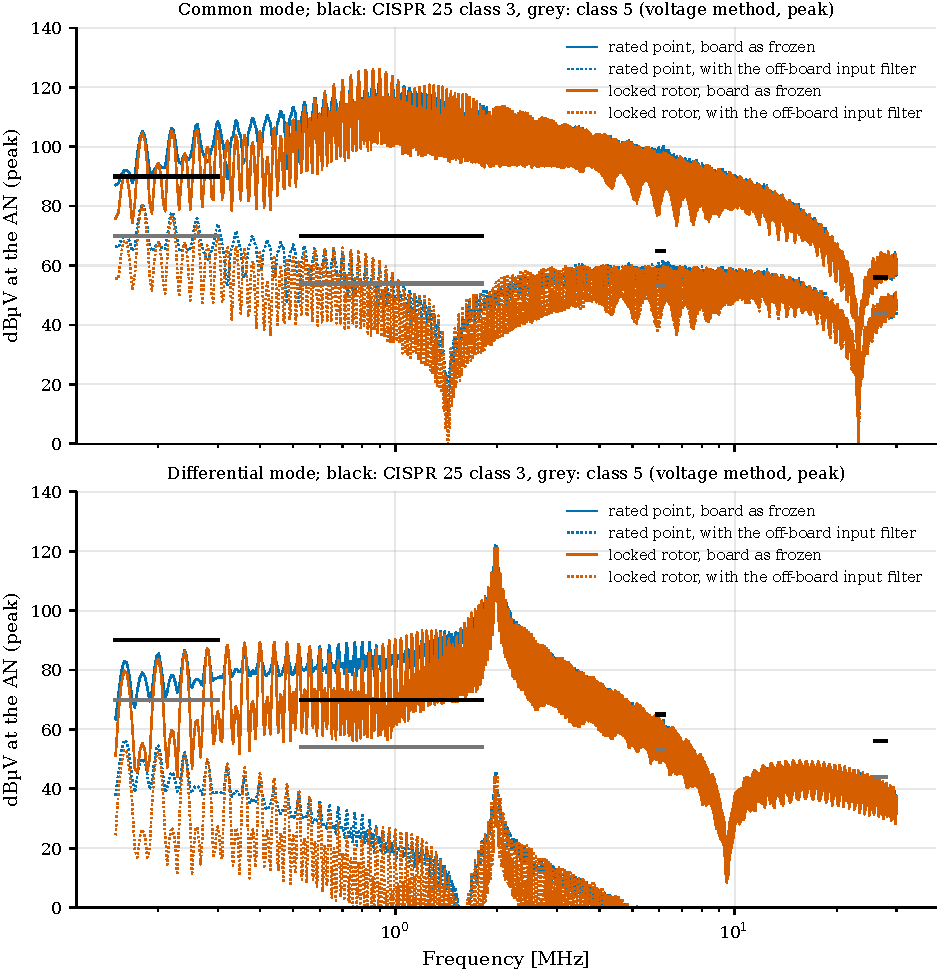
\includegraphics[width=\textwidth]{emc_emc_condotte.pdf}
\caption{Estimated conducted emission at the artificial network, common and
differential mode, rated point and locked rotor, without and with the
off-board input filter of \cref{tab:emcfilter}; class~3 (black) and class~5
(grey) peak limits in the broadcast bands.}
\label{fig:emcest}
\end{figure}

\begin{finding}{The board as frozen needs an input filter, as every unfiltered inverter does}
Without a filter the common mode exceeds class~3 by up to \SI{56}{\decibel}
in the medium-wave band, and the differential mode by \SI{33}{\decibel}. The
numbers are large but not surprising: an \SI{800}{\volt} bridge switching
at \SI{31}{\volt\per\nano\second} into a nanofarad of motor capacitance is a
strong source, and the two \SI{4.7}{\nano\farad} Y-capacitors are the only
return path that does not cross the measurement. The differential-mode
excess sits at the top of the medium-wave band because the film--ceramic
resonance of \cref{sec:complife}, at \SI{2.0}{\mega\hertz}, is just above it.
\end{finding}

\paragraph{The filter, and where it goes.} The model then sizes the filter,
and the first thing it shows is that none of it needs to be on this
board. An input filter between the battery and the DC terminals J101--J102,
in its own compartment of the inverter housing, does the whole job; that is
also where traction inverters usually carry it, on the DC busbars.
%
\begin{itemize}
  \item Common mode: two KEMET SCF39XV-400-2R2B005JH in series,
        nanocrystalline, \SI{0.62}{\milli\henry} each, \SI{40}{\ampere},
        rated \SI{1000}{\volt} AC or DC and qualified to AEC-Q200. One alone
        leaves \SI{3}{\decibel} over the limit in the medium-wave band; two
        give \SI{1.24}{\milli\henry}. Inductance is not the only figure:
        above its self-resonance a choke is a capacitor, and the residual in
        the short-wave and CB bands is set by that capacitance. With
        \SI{20}{\pico\farad} even \SI{2}{\milli\henry} stays \SI{1}{\decibel} above the limit;
        the estimate assumes \SI{10}{\pico\farad} for the pair, which a
        sectored winding reaches, and the choke's datasheet must confirm it.
  \item Differential mode: no separate inductor. The leakage of the
        common-mode chokes, about \SI{1}{\percent} of their inductance, with
        a \SI{1}{\micro\farad} film X-capacitor on the battery side, forms an
        LC filter. An inductor alone works poorly against the
        \SI{100}{\ohm} of the network (\SI{20}{\micro\henry} still leaves
        \SI{18}{\decibel}), while the LC brings the differential mode
        \SI{33}{\decibel} below the limit.
  \item No damper. An RC network across the bus, tuned to the
        film--ceramic resonance, removes \SI{12}{\decibel} on its own; with
        the X-capacitor in place it adds less than \SI{1}{\decibel}, and it
        would have been the only part of the filter on the board. It is
        left out.
\end{itemize}

\begin{table}[htbp]
\centering
\caption{Input EMI filter, outside the board, between battery and the DC
terminals.}
\label{tab:emcfilter}
\small
\begin{tabularx}{\textwidth}{lYY}
\toprule
Part & Choice & Requirement it meets \\
\midrule
CM choke, two in series & KEMET SCF39XV-400-2R2B005JH, \SI{0.62}{\milli\henry}, \SI{40}{\ampere}, \SI{1000}{\volt}, AEC-Q200 &
  \SI{1.24}{\milli\henry} in total; self-capacitance $\leq\SI{10}{\pico\farad}$; bus current \SI{32}{\ampere} with ripple \\
X-capacitor & \SI{1}{\micro\farad}, \SI{1100}{\volt} DC film, AEC-Q200 (Panasonic ECW-FG class) & battery side of the chokes \\
Y-capacitors & the two \SI{4.7}{\nano\farad} on the board & inverter side of the chokes, as they are \\
Cables & shielded DC and motor cables, \SI{360}{\degree} shield termination at the housing &
  the motor capacitance returns through the shield, not through the network \\
\bottomrule
\end{tabularx}
\end{table}

With the filter the estimate is inside class~3 in every band, by at least
\SI{3}{\decibel} (\cref{tab:emcest}). That margin is thin against the
accuracy of an estimate, and the medium-wave band, where the inductance runs
out first, is the one to watch; a third choke is the obvious reserve. Two
side effects are welcome. The leakage of the chokes, about
\SI{12}{\micro\henry}, sits between the battery and the DC-link and meets
requirement R11 from inside the inverter: the source--capacitor resonance of
\cref{sec:dclink} moves to about \SI{3}{\kilo\hertz}, far below the
switching harmonics. And the chokes dissipate about \SI{3}{\watt} at full
current, in the filter compartment and not on the board.

The estimate does not cover what only a built board shows: radiated
emission, coupling between the switching nodes and the harness, the actual
shield termination, and anything above \SI{30}{\mega\hertz}. It does say
how large the filter is, that it fits outside the frozen board, and what it
costs: about \SI{140}{}~EUR on a prototype (\cref{app:bom}).

\section{Insulation coordination}
\label{sec:insulation}

The requirements quoted below come from a third-party calculator that
implements a stored subset of IEC 60664-1~\cite{standardclarity}, not from
the text of the standard~\cite{iec60664}, which was not available. This is a
secondary source: published, reproducible and parameter-addressable, but not
the standard itself, and it describes itself as a reference estimate. Every
case cited here is reproducible from the permalink given in the reference.

It was used to check nine values that had previously been quoted from
memory (five creepage rows, two clearance rows, the reinforced doubling rule
and the pollution-degree floor), and all nine agree to the digit.
That is reassuring about the memory and says nothing about the calculator's
own coverage; the standard is still to be read before release
(\cref{app:assumptions}).

\paragraph{\SI{900}{\volt} is not a row of the tables.} The creepage table
of IEC 60664-1 lists \SI{800}{} and \SI{1000}{\volt}; every creepage value at
\SI{900}{\volt} in this chapter is a \emph{linear interpolation} between
the two, which is what the calculator does and states that it
does~\cite{standardclarity}, rounded up to the next \SI{0.1}{\milli\metre}.
Clearance is treated differently and needs no interpolation at all: it is
selected by rated impulse voltage in discrete steps, and \SI{2.5}{\kilo\volt}
is a row (\SI{1.5}{\milli\metre}; \SI{3.00}{\milli\metre} for reinforced
insulation, taken one impulse step higher, at \SI{4}{\kilo\volt}).
Whether the standard permits interpolating creepage is to be confirmed on
its text. If it did not, the \SI{1000}{\volt} row would apply: in pollution
degree 1, which is the design basis, the drain--source gap would pass by
\SI{1}{\percent} (\SI{3.24}{} against \SI{3.2}{\milli\metre}) and every
other barrier would keep its margin; the pollution-degree-2 checks of
\cref{tab:pd2robust} would each lose \SI{0.5}{} to \SI{1}{\milli\metre}.

\subsection{What the package leaves}

The worst pair is drain to source on a single device, and its separation is
fixed by the package: pads \SI{1.84}{\milli\metre} wide on a
\SI{5.08}{\milli\metre} pitch leave \SI{3.24}{\milli\metre} of bare laminate
at the full bus voltage. The other close pair, at \SI{0.70}{\milli\metre}, is
between source, Kelvin source and gate, which see the gate voltage and not
the bus.

\begin{table}[htbp]
\centering
\caption{Creepage required at the \SI{900}{\volt} working voltage
($V_\mathrm{max,cont}$, \cref{tab:vhierarchy}) against the
\SI{3.24}{\milli\metre} available.}
\label{tab:creepage}
\begin{tabular}{lrrl}
\toprule
Condition & Required & Margin & \\
\midrule
\textbf{Pollution degree 1}, coated & \textbf{\SI{2.80}{\milli\metre}} & $+\SI{16}{\percent}$ & \textbf{passes} \\
PD2, material group I (CTI $\geq$ \num{600}) & \SI{4.50}{\milli\metre} & $-\SI{39}{\percent}$ & fails \\
PD2, material group II & \SI{6.35}{\milli\metre} & $-\SI{96}{\percent}$ & fails \\
PD2, material group IIIa (ordinary FR-4) & \SI{9.00}{\milli\metre} & $-\SI{178}{\percent}$ & fails \\
\bottomrule
\end{tabular}
\end{table}

\subsection{Clearance, and the rule that couples it to creepage}
\label{sec:clearance}

Creepage may not be smaller than clearance. Clearance in turn does not follow
from the working voltage but from the assumed \emph{rated impulse withstand},
so an assumption about impulse can raise the required creepage above the
table value, and the next subsection works out what that means for this
board.

\begin{table}[htbp]
\centering
\caption{Rated impulse, clearance, and the creepage that results in pollution
degree 1, against the \SI{3.24}{\milli\metre} the package leaves.}
\label{tab:impulse}
\begin{tabular}{lrrl}
\toprule
Rated impulse & Clearance & Creepage (PD1) & Margin on \SI{3.24}{\milli\metre} \\
\midrule
\SI{1.5}{\kilo\volt} & \SI{0.50}{\milli\metre} & \SI{2.80}{\milli\metre} & $+\SI{16}{\percent}$ \\
\textbf{\SI{2.5}{\kilo\volt}} (selected) & \SI{1.50}{\milli\metre} & \SI{2.80}{\milli\metre} & $+\SI{16}{\percent}$ \\
\SI{4}{\kilo\volt} & \SI{3.00}{\milli\metre} & \SI{3.00}{\milli\metre} & $+\SI{8}{\percent}$ \\
\SI{6}{\kilo\volt} & \SI{5.50}{\milli\metre} & \SI{5.50}{\milli\metre} & $-\SI{41}{\percent}$: fails \\
\bottomrule
\end{tabular}
\end{table}

At the selected level the air gap (\SI{1.50}{\milli\metre} required against
\SI{3.24}{\milli\metre} available) does not constrain the design, and the
surface path governs, which is what the coating addresses. Clearance stays below creepage only as long as the impulse assumption of
\cref{sec:ovc} holds. Above \SI{4}{\kilo\volt} clearance
becomes the quantity that sets creepage, and the design does not survive
\SI{6}{\kilo\volt}.

\subsection{Overvoltage category does not apply here}
\label{sec:ovc}

IEC 60664-1 coordinates insulation for equipment \emph{within low-voltage
supply systems}. Its rated-impulse table is indexed by the nominal voltage of
the supply system and by the overvoltage category, and the category encodes
one thing: how much the distribution network attenuates a lightning or
switching transient before it reaches the equipment.

This inverter is fed from a traction battery, and the high-voltage system
floats with respect to chassis. During driving it is connected to no
distribution network at all.

During charging it is. The contactors are \emph{closed} while charging,
since that is how the energy reaches the pack, so a conductive path from the inlet to the DC bus exists, with the
inverter sitting on it. What interrupts the mains transient is not the
contactors but the galvanic isolation of the charging equipment: the
high-frequency transformer of the on-board charger in AC charging, or of the
off-board station in DC charging. That is equipment outside this perimeter,
so it becomes a requirement on the system (R10 of \cref{tab:sysreq}) rather
than an assumption buried in a clearance table.

Whether it is normatively guaranteed is less clear. The governing
documents are ISO 17409~\cite{iso17409} on the vehicle side and
IEC 61851-23~\cite{iec6185123} for DC charging stations; neither text was
available here. What is known of their structure settles the question in the
negative: IEC 61851-23 distinguishes isolated from non-isolated DC charging
stations and imposes additional protective measures on the latter, so
galvanic isolation is \emph{not} universally mandated. It is an architecture
assumption, and it is recorded as one.

With that assumption standing, there is no physical path by which a
\SI{6}{\kilo\volt} mains-borne impulse reaches the drain--source gap of a
device, and applying category II would transfer a mains assumption to a
system separated from the mains by a transformer. Without it, the bus is
galvanically tied to the grid while charging, the category applies again, and
the \SI{2.5}{\kilo\volt} declared here would not help: that is not a
transient this board can absorb but a different normative domain, to be
mitigated at the charge inlet rather than on this board.

\begin{finding}{Overvoltage category II would have failed the board}
Selecting the \SI{1000}{\volt} supply band with overvoltage category
II, the combination an engineer trained on mains-connected equipment reaches
for, gives a \SI{6}{\kilo\volt} rated impulse, \SI{5.50}{\milli\metre} of
clearance, and therefore \SI{5.50}{\milli\metre} of required creepage against
\SI{3.24}{\milli\metre} available. The board would fail by \SI{41}{\percent},
and no coating recovers it.

The design survives because the overvoltage category is a category error for
a battery system, not because of a margin. Since that reason sounds fragile,
the room it leaves matters: the design passes up to and including a \SI{4}{\kilo\volt} rated impulse, which
is what category~I on a \SI{1000}{\volt} system would give. It fails only at
category II or worse.
\end{finding}

What replaces the category is the transient that exists on the board, which is
generated inside the converter and has been simulated rather than assumed:
at the \SI{950}{\volt} overvoltage trip and the \SI{60}{\ampere} overload
trip the die sees \SI{1073.5}{\volt} with the \SI{20}{\nano\henry} layout
limit and \SI{1148}{\volt} even at \SI{50}{\nano\henry}, two and a half times
the limit (\cref{tab:overshoot}).

\begin{finding}{Opening a contactor is worth five volts, not kilovolts}
The step from \SI{1.5}{} to \SI{2.5}{\kilo\volt} was originally justified by
a contactor opening into an inductive high-voltage harness, an event that had
never been estimated. Estimating it changes the argument.

Two \SI{50}{\milli\metre\squared} conductors \SI{30}{\milli\metre} apart give
$(\mu_0/\pi)\ln(d/r) = \SI{0.72}{\micro\henry\per\metre}$, so a
\SI{3}{\metre} harness is \SI{2.16}{\micro\henry}. What matters next is the
topology: the DC-link capacitor sits on the \emph{inverter} side of that
harness, so when the contactor opens the harness current continues into
\SI{200}{\micro\farad}. The circuit impedance is
$\sqrt{L/C} = \SI{0.104}{\ohm}$ and the overvoltage is $I\sqrt{L/C}$:
\SI{3.6}{\volt} at \SI{35}{\ampere}, \SI{10.4}{\volt} at \SI{100}{\ampere},
\SI{52}{\volt} if a fuse interrupted \SI{500}{\ampere}. Reaching
\SI{2.5}{\kilo\volt} would take \SI{24}{\kilo\ampere}.

The DC-link capacitor is a formidable clamp for anything arriving along the
harness, and the dominant transient on this board remains the one the board
generates itself.
\end{finding}

\SI{2.5}{\kilo\volt} is declared even so, one step above the
\SI{1.5}{\kilo\volt} that would cover the simulated worst case. The reason is
not the external events, which are now quantified at tens of volts, but what
cannot be quantified: electrostatic discharge at the high-voltage connector
during service, lightning coupling to the vehicle, anything this model does
not contain. It costs nothing, because creepage remains the binding quantity
at \SI{2.80}{\milli\metre} either way, so the figure is \emph{abundant rather
than marginal}: \num{2.2} times the worst internal case and \num{48} times
the worst external event estimated.

\subsection{Two air paths the design rule check cannot see}

Clearance is a distance through air, and two of the air paths that matter run
outside the board copper the design rule check measures.

The tab of the TO-247 package \emph{is} the drain, at up to \SI{900}{\volt}, and it
is clamped against a cold plate at chassis potential. The insulating pad
handles the solid insulation; what had never been dimensioned is the surface
path around the \emph{edge} of the pad, which is a reinforced barrier.

\begin{finding}{The pad is outside the board, so it inherits nothing from the
coating}
Every other distance in this design is qualified in pollution degree 1
because the board is conformally coated. The pad is not on the board: it sits
between the package tab and the cold plate, and that surface is not coated.
Its pollution degree depends on the sealing of the housing (a mechanical
part outside this perimeter), not on our coating process. The two are
independent assumptions, and treating them as one was an error.

The source used here says as much: coating or sealing does not automatically
reduce the pollution degree, and any reduction depends on the protection
method applied~\cite{standardclarity}.
\end{finding}

\begin{table}[htbp]
\centering
\caption{Insulating pad sized by the creepage around its edge. Reinforced
barrier at \SI{900}{\volt}; path available is the overhang plus the
\SI{0.63}{\milli\metre} pad thickness; tab \SI{15.9}{}$\times$\SI{20}{\milli\metre}.}
\label{tab:pad}
\begin{tabular}{lrrl}
\toprule
Microenvironment at the pad & Creepage & Overhang & Pad \\
\midrule
PD1, sealed housing & \SI{5.60}{\milli\metre} & \SI{4.97}{\milli\metre} & \SI{26}{}$\times$\SI{30}{\milli\metre} \\
\textbf{PD2, material group I} (selected) & \SI{9.00}{\milli\metre} & \SI{8.37}{\milli\metre} & \textbf{\SI{33}{}$\times$\SI{37}{\milli\metre}} \\
PD2, material group II & \SI{12.70}{\milli\metre} & \SI{12.07}{\milli\metre} & \SI{41}{}$\times$\SI{45}{\milli\metre} \\
\bottomrule
\end{tabular}
\end{table}

Pollution degree 2 is chosen, and the housing assumption is
dropped. Most automotive housings carry a pressure-equalisation membrane,
which means they breathe and therefore condense; the standard places
occasional condensation explicitly inside pollution degree 2. Buying
independence from a system-level assumption costs \SI{57}{\percent} more pad
area on a component worth a few euro. This is the only point in the whole
insulation coordination where an assumption was \emph{removed} rather than
declared.

The ceramic itself is assigned material group I, which a pad datasheet
stating CTI $\geq \SI{600}{\volt}$ would confirm. Neither alumina nor the
aluminium nitride adopted in \cref{sec:coolalt} tracks, and
the standard is understood to exempt non-tracking inorganic materials from
requiring creepage greater than clearance, which would give
\SI{3.00}{\milli\metre} instead of \SI{9.00}{\milli\metre}. That exemption is
\emph{not} taken: the secondary source available does not implement it, and
the path runs over ceramic veiled in thermal grease, which is organic.

A catalogue part sold as a TO-247 pad is typically
\SI{20}{}$\times$\SI{25}{\milli\metre}, less than a third of the required
area. The pad had been selected on thermal resistance alone
(\cref{tab:rthcs}), where its size never appears. \Cref{tab:pad} sizes a pad
standing on its own; on the cooling rail of \cref{sec:mechanics} the strip
is \SI{35.5}{\milli\metre} tall, and the creepage below the tab is obtained by
raising the rail rather than by extending the ceramic, which gives
\SI{10.1}{\milli\metre} around the edge (\cref{fig:mechsection}).

The thermal chain does not move. Heat enters through the tab and spreads at roughly
\SI{45}{\degree} as it crosses the pad, so the flux widens by about one pad
thickness (\SI{0.63}{\milli\metre}) per side. The overhang is
\SI{8.4}{\milli\metre}, thirteen times that, and therefore lies entirely
outside the spreading cone: it carries no heat. Adding ceramic around the
loaded area cannot increase $\Rthcs$; it can only add a weak parallel path.
The pad's size therefore changes no temperature in this report; its
thermal resistance is set by the material and the interfaces
(\cref{sec:coolalt}).

\begin{finding}{A screw through the tab would short the barrier the pad
creates}
The TO-247 has a mounting hole in its tab, and the tab is the drain at
up to \SI{900}{\volt}. A metal screw passing through it into the cold plate
reduces the creepage path from \SI{9}{\milli\metre} to zero. Clip mounting on the
plastic body is therefore selected, which also gives the uniform pressure
that makes $\Rthcs$ reproducible. If a screw were required for mechanical
reasons, an insulating shoulder bushing and washer would be mandatory
components.
\end{finding}

The cold plate itself, its screws and the surrounding structure are at
chassis potential and sit millimetres from the board, but they are not nets
in the PCB file and no rule can check them. A mechanical clearance of
\SI{5.0}{\milli\metre} from any high-voltage copper is specified, above the
\SI{3.00}{\milli\metre} the standard asks, because this dimension lives in an
assembly with mechanical tolerances rather than in a photoplot.

\begin{finding}{Conformal coating is part of the design}
Conformal coating over the high-voltage area brings the pollution degree from
2 to 1 and the requirement from \SI{9.00}{} to \SI{2.80}{\milli\metre}, a
\SI{69}{\percent} reduction that turns a \SI{178}{\percent} shortfall into a
\SI{16}{\percent} margin. Every insulation distance in this design, the
reinforced barrier included, depends on it.

Without the coating the board is \emph{unbuildable with this device}: \SI{9.00}{\milli\metre} would be
required where the package offers \SI{3.24}{\milli\metre}, and no layout can
recover the difference. The design-rule check cannot see this, since the board
passes either way, so the condition is stated at the head of the rules file
and on the fabrication drawing.
\end{finding}

The reinforced barrier to the control side is set at \SI{8}{\milli\metre},
which is what the components themselves
provide~\cite{ti_ucc21750,ti_amc1302}. Read against IEC 60664-1, where
reinforced insulation requires twice the basic creepage, that is
\SI{5.60}{\milli\metre} in pollution degree 1 and \SI{18}{\milli\metre} in
pollution degree 2 on ordinary FR-4, at \SI{900}{\volt}. The adopted figure
therefore has \SI{43}{\percent} of margin under the coating assumption and
none without it. Saying that this
barrier is ``guaranteed by the components'' is true of the component body and
false of the copper around it.

\subsection{Laminate material group}

The certified creepage of an isolator and the CTI of its body describe the
component. The path that has to be qualified runs on the \emph{laminate},
which is a different material and is ordinarily material group IIIa. The
laminate is therefore specified in its own right, at CTI
$\geq\SI{600}{\volt}$, material group I.

On its own this does not save the drain--source pair (\SI{4.50}{\milli\metre}
required against \SI{3.24}{\milli\metre} available), so it is not an
alternative to the coating. It is a second line of defence, because coating
voids are a known process defect: on ordinary FR-4 a void takes the margin to
$-\SI{178}{\percent}$, on a group I laminate to $-\SI{39}{\percent}$. It is
also the only defence at the board edge, which a coating does not reliably
reach.

\subsection{The board edge, and solid insulation}

Two more paths need checking: around the board edge, and through the solid
insulation between the planes.

Between the DC-positive plane on L1 and the DC-negative plane on L2 the
\SI{0.10}{\milli\metre} prepreg is \emph{solid} insulation, but a second path
exists around the side of the board. Its length is the sum of the two plane
setbacks plus the dielectric. A routed edge is not reliably coated and is
treated as pollution degree 2, where the group I laminate requires
\SI{4.50}{\milli\metre} at \SI{900}{\volt}: the \SI{2.0}{\milli\metre}
setback of the first version gave \SI{4.10}{\milli\metre} and no longer
passes. The rule is now \SI{2.25}{\milli\metre} per plane,
\SI{4.60}{\milli\metre} in all.

The solid insulation itself carries up to \SI{900}{\volt} across
\SI{0.10}{\milli\metre}, a field of \SI{9}{\kilo\volt\per\milli\metre}
against a laminate strength of the order of \SI{30}{}--\SI{40}{\kilo\volt\per\milli\metre}.
It is functional insulation, so no minimum thickness applies (the
\SI{0.4}{\milli\metre} minimum is a reinforced-insulation rule), but this is
the thinnest margin in the design and it cannot be inspected. A
layer-to-layer dielectric withstand test at \SI{2}{\kilo\volt} for one minute
is added to the fabrication drawing, which replaces the assumption with a
measurement.

\subsection{What fails if the coating has a void}

The pad raises a more general question: which barriers survive in pollution
degree 2? With the material group I laminate specified in \cref{sec:insulation}:

\begin{table}[htbp]
\centering
\caption{Barriers against the pollution degree 2 requirement, material group I laminate.}
\label{tab:pd2robust}
\begin{tabular}{lrrl}
\toprule
Barrier & Adopted & Required & Survives? \\
\midrule
Reinforced, HV to control, board copper & \SI{9.5}{\milli\metre} & \SI{9.00}{\milli\metre} & \textbf{yes} \\
Reinforced, isolators: board, around the slot & $\geq\SI{9.5}{\milli\metre}$ & \SI{9.00}{\milli\metre} & \textbf{yes} \\
Reinforced, isolators: package surface & \SI{8.0}{}/\SI{8.5}{\milli\metre} & \SI{9.00}{\milli\metre} & no$^a$ \\
Reinforced, HV to chassis & \SI{9.5}{\milli\metre} & \SI{9.00}{\milli\metre} & \textbf{yes} \\
Functional, HV nodes on the board & \SI{4.5}{\milli\metre} & \SI{4.50}{\milli\metre} & equal$^b$ \\
Functional, drain--source in the package & \SI{3.24}{\milli\metre} & \SI{4.50}{\milli\metre} & no \\
\bottomrule
\multicolumn{4}{l}{\footnotesize $^a$ drivers/amplifiers; a property of the certified component, \cref{sec:isoslot}.} \\
\multicolumn{4}{l}{\footnotesize $^b$ exact equality, declared: see the text below the table.}
\end{tabular}
\end{table}

\begin{finding}{At \SI{900}{\volt} a coating void can reach the reinforced barrier}
At \SI{800}{\volt} the \SI{8}{\milli\metre} taken from the isolator bodies
coincided exactly with what pollution degree 2 requires of a reinforced
barrier on a group I laminate, and the safety barriers held with no coating
at all. At the \SI{900}{\volt} working voltage the requirement is
\SI{9.0}{\milli\metre}. The board copper can follow, and the rule is set at
\SI{9.5}{\milli\metre}; under the isolators a slot takes the board path out
of the question (\cref{sec:isoslot}), and what remains is the surface of the
isolator packages themselves, \SI{8.0}{} and \SI{8.5}{\milli\metre}.

Elsewhere what fails is functional insulation, and, once the board rule is
raised to \SI{4.5}{\milli\metre}, only inside the six small areas occupied
by the device pads, where the \SI{5.08}{\milli\metre} lead pitch leaves
\SI{3.24}{\milli\metre} that no rule can widen.

Raising the board rule costs nothing, because lateral separation does not
open the commutation loop, which closes vertically. The design-rule file
carries the exception as a named area over the pad rows rather than lowering
the threshold everywhere, so that a violation anywhere else is still
reported.
\end{finding}

\paragraph{Two equalities, treated differently.} In the first version of
\cref{tab:pd2robust} two barriers met their requirement exactly, and a
margin of zero protects nothing: the drawn gap survives only if every
fabrication tolerance breaks favourably, and the requirement itself is an
interpolation. The reinforced rules are raised from \SI{9.0}{} to
\SI{9.5}{\milli\metre}, because their failure is an electric-shock hazard
and the half millimetre costs only board area. The functional rule
stays at \SI{4.5}{\milli\metre} and is declared as an exact equality in
pollution degree 2: its design basis is pollution degree 1, where the
requirement is \SI{2.80}{\milli\metre} and the margin \SI{61}{\percent};
the pollution-degree-2 row is a check of what a coating void would do, and
its failure is a functional one, not a safety one. Raising it would buy
robustness against a double fault (a void \emph{and} an adverse
tolerance) at the price of loop area around the power stage.

\subsection{Why milling a slot was rejected}

A through slot between the drain and source pads would lengthen the surface
path without touching the pitch, and it was considered. It was rejected
because a through slot cuts L1 \emph{and} L2, forcing the return current to
travel around it instead of directly beneath the outgoing current. By
\cref{eq:planepair} that term is proportional to the separation between go
and return, so a detour of a few millimetres takes the plane pair from
\SI{0.19}{\nano\henry} to between \SI{6}{} and \SI{23}{\nano\henry}, the
whole board-attributable budget of \cref{tab:loopbudget}, spent to solve a
problem the coating solves for nothing. The slot would also have to be long
to be effective, since the copper here is a \SI{10.4}{\milli\metre} pour
rather than a track, and a milled wall is not reliably coated in any case.

This is the one place where the insulation constraint and the commutation
loop conflict; elsewhere they do not.
The loop closes \emph{vertically} through \SI{0.10}{\milli\metre} of prepreg
while creepage is measured \emph{laterally} along a surface, so widening a
lateral gap does not open the loop. The two devices of a leg are the most
extreme case: the high-side source and the low-side drain are the same net,
so there is no insulation requirement between them at all and they can be
placed as close as the cold plate allows.

\subsection{The slot that is made: under the isolators}
\label{sec:isoslot}

The slot rejected in the previous subsection sat between drain and source,
inside the commutation loop. A slot under each of the seven drivers and four
isolated amplifiers is a different object, and it is made. The two cases
differ in the three respects that decided the first:

\begin{table}[htbp]
\centering
\caption{The two slots against the criteria that decide them.}
\label{tab:slotcompare}
\small
\begin{tabularx}{\textwidth}{lYY}
\toprule
 & Drain--source slot (rejected) & Isolator slot (adopted) \\
\midrule
Barrier & functional & \textbf{reinforced} \\
Position & inside the commutation loop: cuts L1 and L2 & outside every current path:
  no net crosses an isolation barrier, so nothing crosses the slot \\
Failure it prevents & functional (a flashover between two HV nodes) &
  \textbf{safety} (high voltage reaching the control side) \\
Cost & \SIrange{6}{23}{\nano\henry} of loop inductance & board area and a routing
  operation \\
\bottomrule
\end{tabularx}
\end{table}

\paragraph{How the standard counts a through slot.} A groove or slot
counts in the creepage path only if it is at least $X$ wide: \SI{0.25}{},
\SI{1.0}{} and \SI{1.5}{\milli\metre} in pollution degrees 1, 2 and 3,
narrower grooves being bridged as if absent (IEC 60664-1, as reported in~\cite{ti_slup419}). A \emph{through}
slot does not lengthen the surface path, it interrupts it: there is no
surface across it, so the creepage path has to go around its ends, and the
air gap across it becomes a clearance. Two consequences follow. The
clearance to meet across the slot is the reinforced one, \SI{3.00}{\milli\metre}
at the \SI{4}{\kilo\volt} step, not the \SI{1.5}{\milli\metre} of basic
insulation; it is met anyway, because the air path between the pin rows is
unchanged at \SI{8.1}{\milli\metre} or more. And the slot must be long
enough that the path around its ends meets the creepage rule. A blind
groove would count by its contour instead, but on a six-layer board it
would expose inner copper; a through slot is the standard routing
operation and the one specified.

\paragraph{The footprint was wrong before the slot was.} Sizing the slot
required the real copper-to-copper gap under the isolators, and it is not
the \SI{8}{\milli\metre} quoted until now. With the standard
IPC-7351 footprint assigned in the library, the driver pad rows are
\SI{7.25}{\milli\metre} apart: the pads reach under the body. The
manufacturer publishes a high-voltage land pattern for the same package,
with shorter pads on wider rows, that leaves
\SI{8.1}{\milli\metre}~\cite{ti_ucc21750}; the driver footprint is
therefore replaced by it. The amplifiers' footprint leaves
\SI{8.85}{\milli\metre}.

\begin{table}[htbp]
\centering
\caption{Slot dimensions. Path around the slot end from the outermost pad
corner on one side to the other: $2\sqrt{e^2 + (g/2 - w/2)^2} + w$, with
$g$ the gap between pad rows, $w$ the slot width, $e$ the overhang beyond
the outermost pad.}
\label{tab:slotdims}
\begin{tabular}{lrr}
\toprule
 & Drivers (7) & Amplifiers (4) \\
\midrule
Package, creepage over the surface & \SI{8.0}{\milli\metre} & \SI{8.5}{\milli\metre} \\
Pad-row gap $g$ & \SI{8.1}{\milli\metre} & \SI{8.85}{\milli\metre} \\
Slot width $w$ & \SI{1.5}{\milli\metre} & \SI{1.5}{\milli\metre} \\
Pad to slot edge & \SI{3.3}{\milli\metre} & \SI{3.7}{\milli\metre} \\
Slot length & \SI{14.5}{\milli\metre} & \SI{8.5}{\milli\metre} \\
Overhang beyond the outermost pad $e$ & \SI{2.5}{\milli\metre} & \SI{2.0}{\milli\metre} \\
Path around the end & \SI{9.8}{\milli\metre} & \SI{9.9}{\milli\metre} \\
Against the \SI{9.5}{\milli\metre} rule & $+\SI{3}{\percent}$ & $+\SI{4}{\percent}$ \\
\bottomrule
\end{tabular}
\end{table}

The width is \SI{1.5}{\milli\metre}: above the \SI{1.0}{\milli\metre}
minimum with room for the router tolerance, and narrow enough to leave
\SI{3.3}{\milli\metre} to the pads, above the \SI{2.25}{\milli\metre}
setback that the rules apply to any milled edge.

\paragraph{The planes.} The slot must not lengthen a return path, which is
what disqualified the drain--source slot. It cannot, provided it lies
entirely inside the \texttt{KEEPOUT\_BARRIERA} area, which is drawn on
every layer: no plane on L3 or L5 crosses an isolation barrier, by
definition, and the gate loop of each driver (output, gate, Kelvin source
and back to the driver's own reference) lies wholly on the floating side.
The condition is checkable: the slot outline must stay at least
\SI{1}{\milli\metre} inside the keepout on every layer.

\paragraph{Mechanics.} Eleven slots of \SI{1.5}{\milli\metre} under
soldered bodies do not load the joints: the gull-wing leads are compliant,
and the body spans the slot without resting on the board. The risk is
elsewhere. The drivers sit in a row along the barrier, with their slots
aligned on it, and a row of slots is a perforation: under vibration the
board would flex along that line. The rule is that the slots may occupy at
most half the length of the line they lie on (a driver pitch of at least
\SI{29}{\milli\metre}), or that a fixing point stands between groups of
slots, with rounded slot ends (radius $w/2$) and at least
\SI{3}{\milli\metre} from any hole or board edge.

\paragraph{What the slot does not do.} It does not make the reinforced
barrier independent of the coating. With the board path taken away, the
shortest path under each isolator is the surface of its own package,
\SI{8.0}{\milli\metre} for the drivers and \SI{8.5}{\milli\metre} for the
amplifiers, against \SI{9.0}{\milli\metre} in pollution degree 2. That is a
property of a certified component (reinforced to a \SI{2121}{\volt}
working voltage under its own
standard~\cite{ti_ucc21750,ti_amc1302}), and the equipment standard, not the
layout, decides whether it is accepted in pollution degree 2. What the slot
does is remove the one board surface that the coating reaches least
reliably (the gap under a low-standoff body, where the coating does not
flow and cannot be inspected) and leave the barrier on package surfaces
that are exposed, coated and visible.

\begin{finding}{The isolated supplies are not a reinforced barrier at \SI{900}{\volt}}
Checking the isolators led to the other components that cross the same
barrier: the eleven isolated DC/DC converters that supply the drivers and
the sensing. Their datasheet is explicit. As a safety barrier they are
recognised for reinforced insulation up to a working voltage of
\SI{150}{\volt} rms and for basic insulation up to \SI{300}{\volt} rms,
with \SI{2}{\milli\metre} of creepage and clearance; the \SI{5.2}{\kilo\volt}
in their title is a one-second production test, and continuous voltages up
to \SI{2.4}{\kilo\volt} are sustained only as \emph{functional}
insulation~\cite{murata_mgj2}. At \SI{900}{\volt} they are a functional
barrier, not a safety one.

This is independent of the slot and of the coating: it is the component,
not the board. The reinforced barrier between high voltage and
control, as specified, is not met at the supplies. Either they are
replaced by supplies rated for reinforced insulation at a working voltage of
at least \SI{900}{\volt} DC, or the safety barrier is placed elsewhere and
the board's HV-to-control insulation is declared functional. The choice
changes the bill of materials and the insulation concept, and is recorded
as an open decision (\cref{app:assumptions}, A.25).
\end{finding}

\subsection{Fabrication requirements}

\begin{enumerate}
  \item FR-4 laminate, CTI $\geq \SI{600}{\volt}$ (IEC 60112), material
        group I~\cite{iec60112}, $T_g \geq \SI{150}{\celsius}$.
  \item Conformal coating on both faces over the high-voltage area, masked at
        connectors and test points; pollution degree 1 is declared on this
        basis. The coating carries a UV tracer, and every board is
        inspected under UV light over the whole high-voltage area, with
        acceptance on complete coverage of the barrier outlines and of the
        exposed faces of the isolator packages. This turns the coating from
        a process assumption into a verified property of each board, and it
        benefits every barrier, not only the reinforced one.
  \item Through slots \SI{1.5}{\milli\metre} wide under the seven drivers
        (\SI{14.5}{\milli\metre} long) and the four isolated amplifiers
        (\SI{8.5}{\milli\metre}), with rounded ends, per
        \cref{tab:slotdims}; drivers on the manufacturer's high-voltage land
        pattern.
  \item L1--L2 prepreg \SI{0.10}{\milli\metre}; dielectric withstand test
        L1--L2 at \SI{2}{\kilo\volt} DC for one minute.
  \item \SI{2}{oz} outer copper, \SI{1}{oz} inner; finished thickness
        \SI{1.6}{\milli\metre}.
  \item IPC-6012~\cite{ipc6012} class 2 minimum.
  \item Depanelisation before coating; if it followed coating, the board
        edge would be bare and the \SI{2.25}{\milli\metre} setback applies.
\end{enumerate}

These requirements are written on the board file itself, as fabrication
notes on its drawing layer, and leave with the Gerber files; the fabrication
package also carries an assembly drawing, which is what settles the
reference of a part where the silkscreen is crowded.

\subsection{Two limits set by the package}
\label{sec:packagelimits}

\begin{finding}{The TO-247-4L limits both the loop inductance and the
switching frequency}
Two ceilings in this design come from the same component. They were derived
in different chapters, but they are related.

The first is inductance. The two packages of a leg contribute
\SI{14.6}{\nano\henry} that no layout can remove (\cref{sec:kelvin}), against
a board-attributable limit of \SI{20}{\nano\henry}: \SI{73}{\percent} of the
budget is spent before a single track is drawn, and it is this inductance,
through the gate resistance it forces, that makes switching half of the
loss budget. A power module is the only
way past it (\cref{ch:conclusions}).

The second is frequency. IEC 60664-4~\cite{iec606644} derates clearance and
creepage above \SI{30}{\kilo\hertz}. At $\fsw = \SI{20}{\kilo\hertz}$ it does
not apply, but the switching-frequency sweep of \cref{tab:sweep-fsw} reaches
exactly \SI{30}{\kilo\hertz}, and the drain--source creepage has
\SI{16}{\percent} of margin at \SI{900}{\volt} that a derating would
consume. The
\SI{3.24}{\milli\metre} is fixed by the pad pitch and cannot be widened.

Read together they say the same thing. The case for raising the
switching frequency is that it shrinks the DC-link capacitor and the output
filter. But raising it increases switching loss in proportion, and that loss
is already inflated by the \SI{14.6}{\nano\henry} of package inductance;
and past \SI{30}{\kilo\hertz} the insulation coordination has to be redone
with less creepage than the package can give. The discrete TO-247-4L
therefore bounds the design in both directions at once, and a power module
with an integrated busbar would lift both ceilings together: lower package
inductance, and creepage set by the module's own certified geometry rather
than by a \SI{5.08}{\milli\metre} lead pitch.
\end{finding}

\section{Cooling rail and mechanical integration}
\label{sec:mechanics}

The thermal chain of \cref{ch:thermal} assumes each tab pressed on a
liquid-cooled plate through a ceramic pad, and the insulation coordination
puts a reinforced barrier between them. Neither had been drawn. Drawing it
changed the board, which is the reason it was done \emph{before} revision
1.1 was frozen rather than after.

\paragraph{Concept.} The devices stand vertically with the tab towards the
high-voltage side, so the cold plate is a rail: an aluminium
extrusion with six coolant ports running along the row of seven devices
(their design is in \cref{sec:cooling}),
at chassis potential, longer than the board and fixed to the enclosure
beyond its edges, where the coolant fittings are also kept away from the
high-voltage area (\cref{fig:mech3d}). Aluminium nitride, with a phase-change interface material on both faces,
separates tabs and rail (\cref{sec:coolalt}). It is laid in four segments, one
\SI{70}{\milli\metre} long under each leg and one of \SI{35}{\milli\metre} under the
discharge device, because ceramic substrates are not made
\SI{345}{\milli\metre} long; each segment overhangs the tabs by
\SI{12}{\milli\metre} at its ends, more than the \SI{9}{\milli\metre} of
creepage the reinforced barrier needs, and \SI{20}{\milli\metre} of rail
separate one segment from the next. One spring clip per device hooks over the rail and presses
the plastic body, never the tab, which is the drain; this is the clip
mounting selected in \cref{sec:insulation}. The \SI{50}{\watt} discharge
resistor is screwed to the top of the rail, which is where its
\SI{81}{\joule} pulse finds a heat sink.

\begin{figure}[htbp]
  \centering
  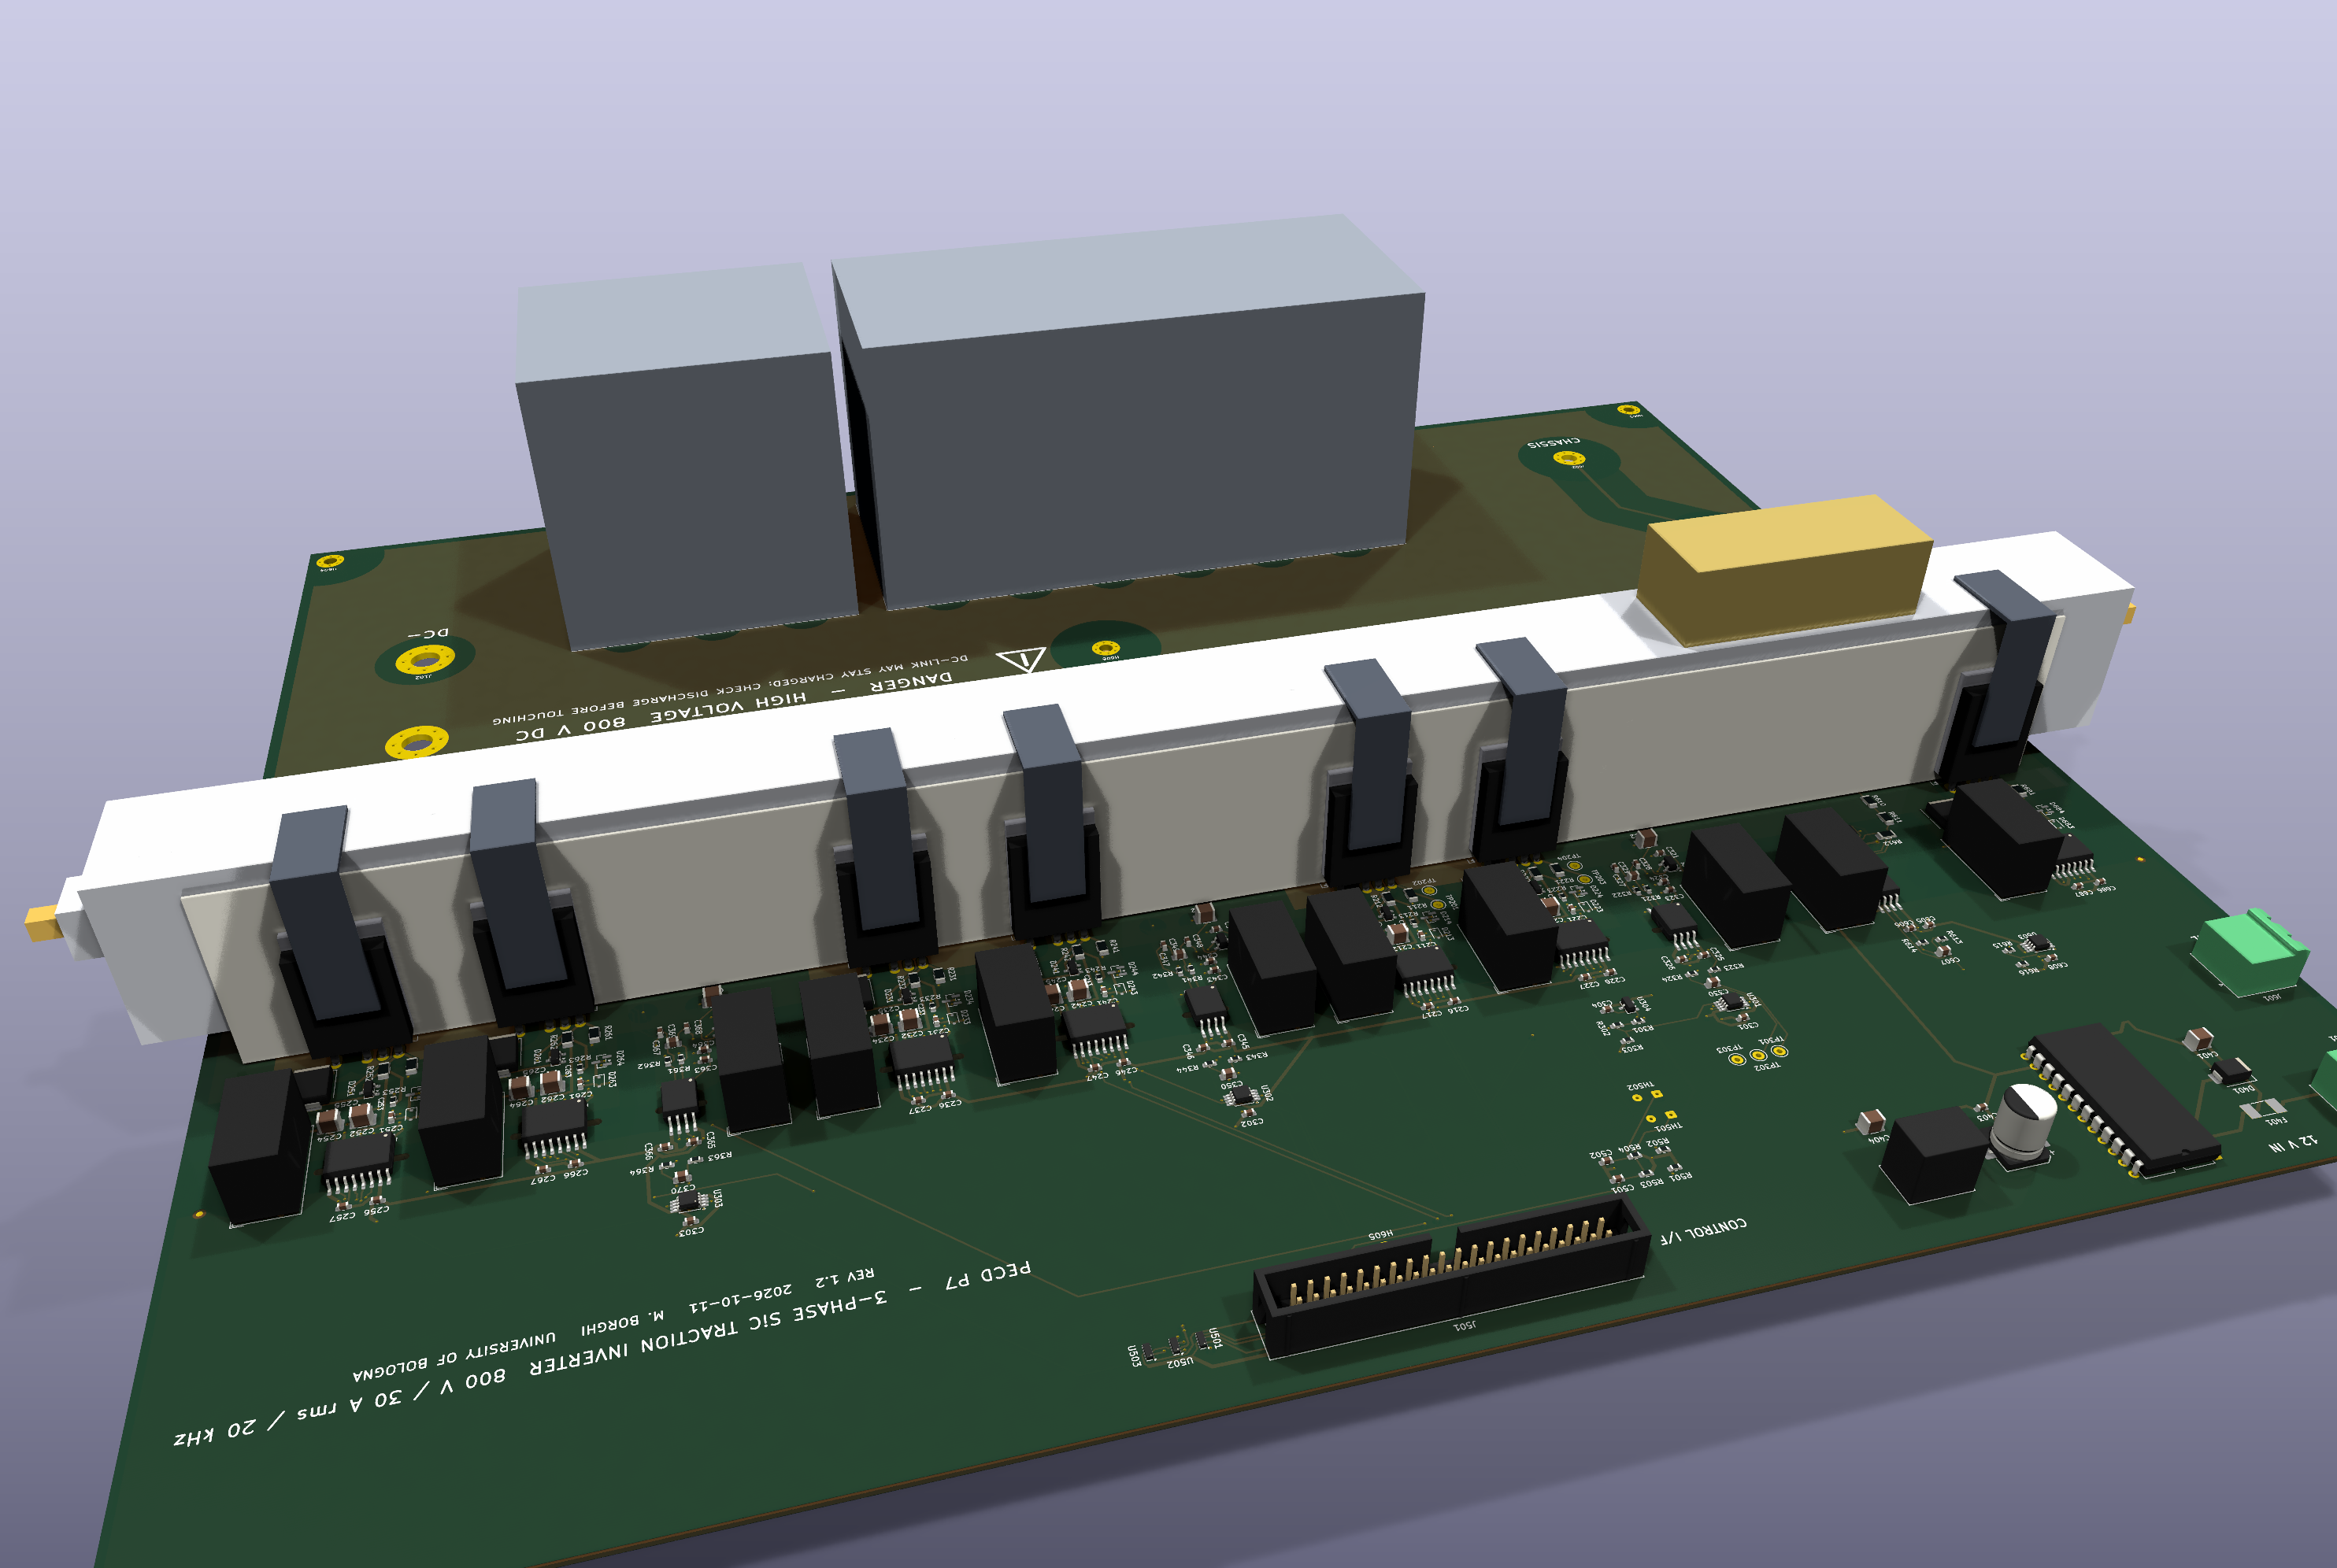
\includegraphics[width=\textwidth]{figures/kicad_meccanica_3d_nord.png}
  \caption{Cooling rail, insulating strip and spring clips on the frozen board,
  seen from the driver side (indicative bodies; the discharge resistor is
  the block on top of the rail).}
  \label{fig:mech3d}
\end{figure}

\paragraph{The profile is set by two distances.} The rail is chassis, so it
must keep \SI{5}{\milli\metre} of air from every high-voltage conductor;
and the creepage from tab to rail around the edge of the pad must reach the
\SI{9.0}{\milli\metre} of a reinforced barrier in pollution degree 2. The
pad cannot extend below the board, so the second condition is met by
raising the rail instead: its lip starts \SI{7.5}{\milli\metre} above the
board, and the path down the pad, under its edge and up to the rail is
\SI{10.1}{\milli\metre} (\cref{fig:mechsection}). The price is that the tab
touches the rail over \SI{81}{\percent} of its height; the uncovered strip
is the lowest \SI{4.5}{\milli\metre}, and the tab, two millimetres of
copper, spreads the heat into the contact area. The lip is
\SI{7}{\milli\metre} thick so that it passes beside the commutation
ceramics; the wide part with the channels starts \SI{13}{\milli\metre} up,
above everything on the board.

\begin{figure}[htbp]
  \centering
  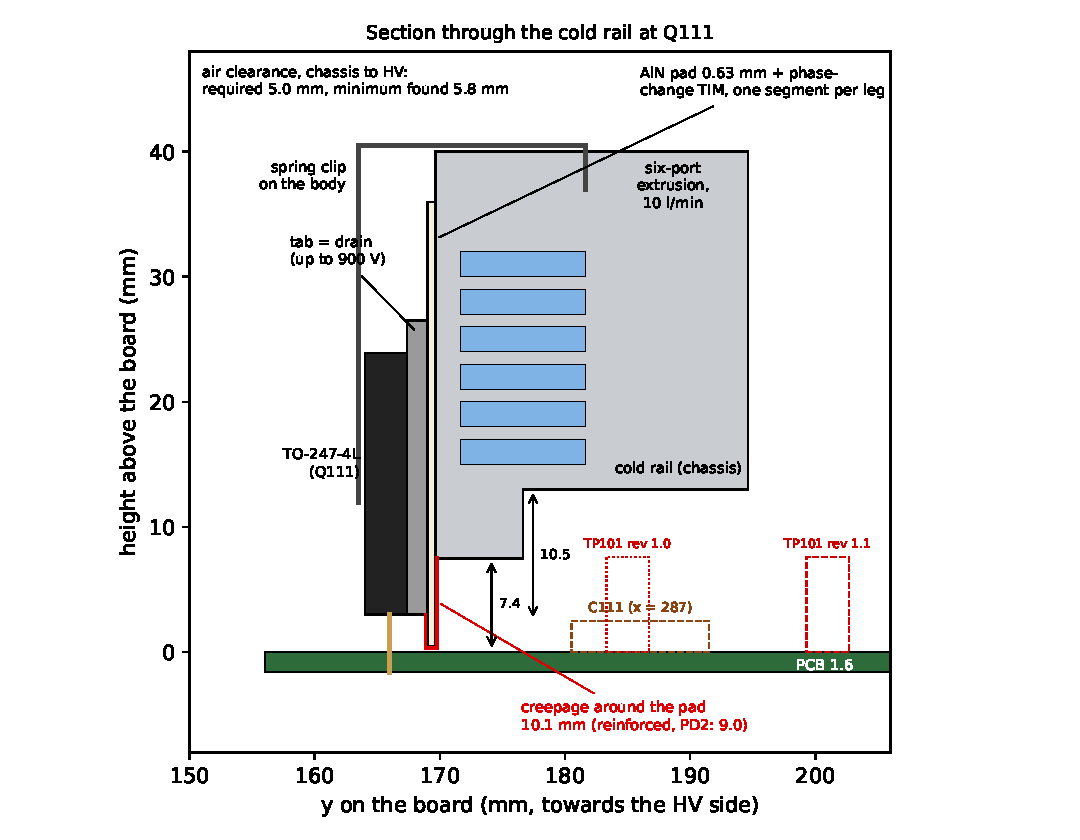
\includegraphics[width=0.92\textwidth]{figures/kicad_meccanica_sezione.pdf}
  \caption{Section through the rail at the high-side device of leg~1, with
  the creepage path around the pad and the two air clearances that set the
  profile. Dashed: parts behind the section plane.}
  \label{fig:mechsection}
\end{figure}

\paragraph{What the check found.} Every chassis part was checked in three
dimensions against every component and copper area of a high-voltage or
floating net, with component heights from their datasheets. The first
profile failed twice: the gate test points of leg~1, \SI{7.6}{\milli\metre}
tall, stood \SI{4.45}{\milli\metre} from the rail, and the commutation
ceramics passed with \SI{0.3}{\milli\metre} of margin. Revision 1.1 moves
the test points \SI{1.5}{\milli\metre} away and moves the switching-node test
point out from under the rail, where no probe could reach it; the profile
was thinned and raised. All parts now keep at least
\SI{5.8}{\milli\metre} of air. The rail, pad and clip outlines are drawn on
the board's documentation layer, so the assembler sees them.

\paragraph{Assembly order.} The devices are soldered \emph{after} they are
clamped to the rail. Soldered first, the leads would carry every tolerance
between the hole pattern and the rail, and the joints of a
\SI{20}{\milli\metre}-tall package would crack at the first thermal cycles.

\section{Design rules as implemented}
\label{sec:rules}

The distances of \cref{sec:insulation} are only as good as the check that
enforces them, and KiCad checks what its rules file says~\cite{kicad10}.
The file translates the coordination into constraints between net classes
(\cref{tab:netclasses}) and named areas, ordered so that every exception
comes after the rule it corrects; \cref{tab:rules} gives the ones that
carry the insulation concept.

\begin{table}[htbp]
\centering
\caption{Design rules that implement the insulation coordination.}
\label{tab:rules}
\small
\begin{tabularx}{\textwidth}{Ylr}
\toprule
Between & Insulation & Clearance \\
\midrule
two different high-voltage nets & functional & \SI{4.5}{\milli\metre} \\
\quad exception: drain and source inside the package area & functional & \SI{3.2}{\milli\metre} \\
\quad inner layers: negative plane to other HV nets and high-side domains (rev.~1.1) & functional & \SI{2.25}{\milli\metre} \\
\quad intermediate nodes of divider and bleeder & functional & \SI{1.6}{\milli\metre} \\
a floating domain and any high-voltage net other than its own reference & functional & \SI{4.5}{\milli\metre} \\
a floating domain and its own reference & --- & \SI{0.2}{\milli\metre} \\
two different floating domains & functional & \SI{4.5}{\milli\metre} \\
high voltage or a floating domain and the control side & reinforced & \SI{9.5}{\milli\metre} \\
\quad exception: the two pad rows of an isolator & reinforced, component & \SI{8.0}{\milli\metre} \\
\quad exception: the pins of an isolated supply (A.25) & functional & \SI{5.5}{\milli\metre} \\
a net that matches no class and anything hazardous & reinforced & \SI{9.5}{\milli\metre} \\
chassis, and the fixing holes, and anything hazardous & reinforced & \SI{9.5}{\milli\metre} \\
hazardous copper and the board edge & functional & \SI{2.25}{\milli\metre} \\
any copper under an isolator body & --- & forbidden \\
\bottomrule
\end{tabularx}
\end{table}

\paragraph{What changed while the board was laid out.} Five rules were
added or corrected once real copper existed, each found by the board rather
than by the analysis.
\begin{itemize}
  \item \emph{One class per domain} (\cref{ch:schematic}): a single class for
        all gate domains made the gate and the Kelvin source of the same
        device a violation.
  \item \emph{Unused pins.} KiCad gives every unused pin a net of its own;
        the rules first read those nets as unclassified, hence low voltage,
        and demanded \SI{9.5}{\milli\metre} between the pins of one package.
        They are now treated as having no net.
  \item \emph{Fixing holes.} The six M3 holes have no net, because the screw
        is earthed through the enclosure and not through the board; without a
        net they fell under the no-net rule, \SI{0.15}{\milli\metre}. A rule
        placed after it gives them the chassis distance back, and the copper
        of the positive rail stops \SI{10}{\milli\metre} from them.
  \item \emph{Width warnings.} The two signal-level connections on power nets
        are exempted by name and by area, as described under conductor
        sizing, so that a warning on those nets always means a real
        conductor.
  \item \emph{Inner layers} (revision 1.1). A surface creepage applied inside
        the laminate cost a third of the commutation loop
        (\cref{sec:loopextract}); the inner-layer value of IPC-2221B
        replaces it for the negative plane only.
\end{itemize}

\paragraph{The rules are themselves tested.} A rule with a syntax error is
silently ignored by the command-line checker, and a rule with a wrong
condition passes everything. A test board places the project's own
footprints on their real nets, once correctly and once in each wrong way,
and the check must report exactly the rule expected for each wrong case and
nothing for the correct ones; it is run after every change to the rules file.

\section{Verification and freeze}
\label{sec:freeze}

The board was first frozen on 11 October 2026 as revision 1.0, and the same
day again as revision 1.1, after the extraction and the mechanical
check had found what the design rule check could not: the phase-pour neck,
the cost of the clearance holes, and the test points too close to the rail.
Revision 1.1 changes copper and test-point positions only; the circuit is
the same. Each revision is recorded together with the exact files its
checks (\cref{tab:freeze}) were run on.

Revision 1.2 adds only what the fabricator and the assembler need:
three fiducials for automatic placement, a box for the serial number, a
drawing of the areas to mask before coating, and assembly notes (the
bleeders raised off the board, \cref{sec:complife}; the devices clamped to the
rail before they are soldered). No signal or power copper moves. Writing the
rule that keeps the fiducials, copper without a net, \SI{9.5}{\milli\metre}
from high voltage exposed a behaviour of the rule engine: a
clearance set locally on a pad (the library fiducial carries one) overrides
the custom rules, so the new rule stayed silent until the test board was made
to violate it. The local value was removed and the test board now carries the
case.

\begin{table}[htbp]
\centering
\caption{Checks passed by the frozen board.}
\label{tab:freeze}
\small
\begin{tabularx}{\textwidth}{lY}
\toprule
Check & Result \\
\midrule
Design rule check, all severities, zones refilled & 0 violations, 0 unconnected items \\
Board against schematic & 0 differences \\
Schematic against the independent model & 275 of 275 parts, pin by pin \\
ERC & one warning, intended (\cref{ch:schematic}) \\
Rules test board & every case as expected, 19 track cases among them \\
Routing checks, project script & 8 of 8: no track on the ground planes or inside the negative plane;
  no track on the wrong side of the barrier; class widths; gate loop
  $\leq\SI{25}{\milli\metre}$ in every channel; sensing pairs coupled \\
Geometry & 2168 segments, all at \SI{0}{}, \SI{45}{} or \SI{90}{\degree} \\
Commutation loop, extracted & \SI{7.8}{\nano\henry} of copper per leg, about
  \SI{8.3}{\nano\henry} with ESL, against the \SI{20}{\nano\henry} limit (\cref{sec:loopextract}) \\
Gate loop, extracted & \SI{13}{\nano\henry} of copper; die peak \SI{1040}{\volt} in the double pulse \\
Mechanics & every chassis part $\geq\SI{5.8}{\milli\metre}$ of air from HV; creepage around
  the pad \SI{10.1}{\milli\metre} (\cref{sec:mechanics}) \\
Silkscreen & every reference visible, upright, \SI{1.0}{\milli\metre} high
  (\SI{0.8}{\milli\metre} where crowded), stroke \SI{0.15}{\milli\metre},
  off the pads and nearer to its own part than to any other \\
Board markings & name, revision, HV warning with a warning triangle,
  terminal and connector labels \\
Fabrication outputs & Gerber, drill, placement, bill of materials,
  assembly drawing: generated by script, after a blocking rule check \\
\bottomrule
\end{tabularx}
\end{table}

What the freeze does \emph{not} settle is listed where it belongs: the
\emph{measured} loop inductance, which the extraction predicts but does not
replace (A.14), and the reinforced rating of the isolated supplies (A.25).

\subsection{Planned for later revisions}
\label{sec:nextrev}

The frozen board is the exam design. What a production version would change
is listed here, in the order it would be done.

\begin{itemize}
  \item Reinforced auxiliary supplies and a discharge that survives
        the loss of \SI{12}{\volt} (A.25, A.L1): a revision of the auxiliary
        supply, with new modules and footprints.
  \item Automotive-qualified replacements for the parts that are not:
        isolated converters, the \SI{12}{\volt} pre-regulator, connectors,
        the transient suppressor, the fuse.
  \item Four layers instead of six (\cref{sec:stackup}): the negative
        DC plane and the ground planes share one inner layer, the
        \SI{1.2}{\metre} of control tracks on L2 move to the remaining signal
        layer. The commutation loop does not change, since the plane stays
        \SI{0.10}{\milli\metre} under L1. Estimated saving about \SI{120}{}~EUR
        per board on a prototype run and \SI{40}{}~EUR in series of a hundred,
        the whole of it in the bare board; best done together with moving the
        film capacitors onto a laminated busbar off the board.
  \item Internally isolated TO-247-4 power devices once one is
        offered at this resistance with automotive qualification
        (\cref{sec:coolalt}): same footprint, no external pad.
  \item The input EMI filter of \cref{tab:emcfilter}, outside the
        board between battery and DC terminals: two \SI{0.62}{\milli\henry}
        common-mode chokes in series, whose leakage serves the differential
        mode, and a \SI{1}{\micro\farad} X-capacitor. The board does not
        change for it; the measurement confirms it once the limit class is
        fixed (A.19).
  \item The bill of materials of \cref{app:bom}, redone on the
        production revision.
\end{itemize}
